\chapter*{第五部分:运动}
% Movement 是指从静止状态变成运动的状态,是一个生物的身体的任何一个部位或是器官,包括自发的和非自发的,自发的如行走时肌肉的运动等,非自发的如心跳等
% 移动(Locomotion)
% 运动(Motion)是广义的,包含一切肢体、部件的动作。
\markboth{总论}{总论}

\begin{figure}[htbp]
	\centering
	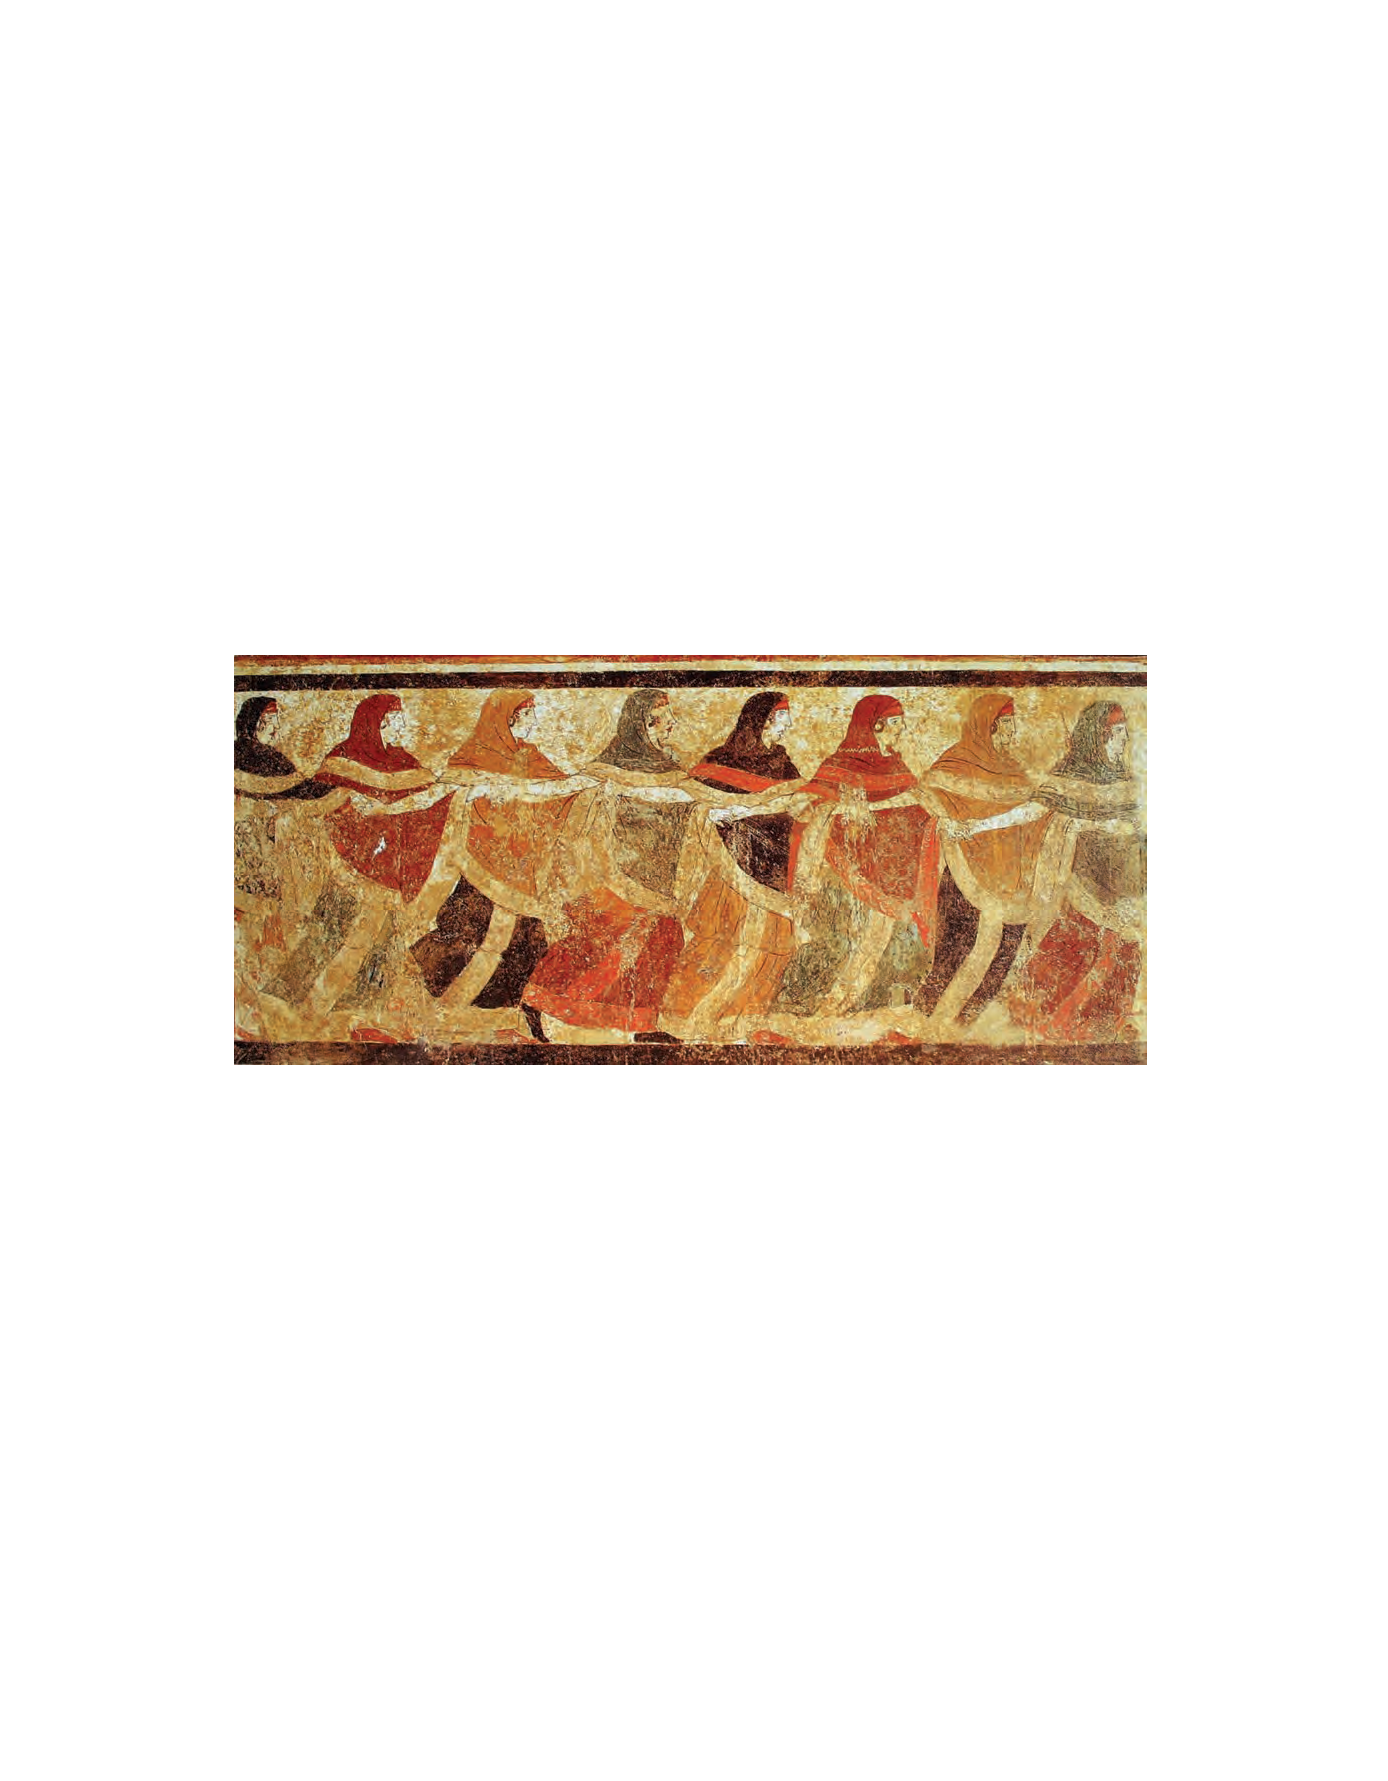
\includegraphics[width=1.0\linewidth]{chap30/fig_30_0}
	\caption{公元前4-5世纪,鲁沃迪$\cdot$普利亚科索科图加诺墓地舞蹈家陵墓中的\href{https://en.wikipedia.org/wiki/Tomb_of_the_Dancers}{舞蹈家妇女壁画}。
		这座陵墓有半室的设计。
		它的六块彩绘面板描绘了30名跳舞的女性,她们从左到右移动,双臂交叉,仿佛她们在坟墓内部绕着圆圈跳舞。
		墓中死者的遗骸显然属于一位杰出的男性战士。
		陵墓以墓中壁画上出现的舞女命名。
		带有壁画的展板现陈列在那不勒斯国家考古博物馆。 }
	\label{fig:30_0}
\end{figure}


正如许多词典提醒我们的那样,运动能力是动物生命的一个决定性特征。
正如运动系统研究的先驱谢灵顿所指出的那样,“人类所能做的就是移动物体,因为无论是在轻声说出一个音节还是在砍伐森林,唯一的执行者都是肌肉。”


人类能够进行的大量运动源于大约 640 块骨骼肌的活动,这些骨骼肌都在中枢神经系统的控制下。
大脑和脊髓的运动中心在处理了有关身体及其周围环境的感觉信息后,会发出神经命令,从而实现协调、有目的的运动。


运动系统的任务与感觉系统的任务相反。
感觉处理在大脑中产生外部世界或身体状态的内部表征。
运动处理从内部表示开始:运动的预期目的。
然而,至关重要的是,这种内部表示需要通过内部生成的信息(有效副本)和外部感觉信息不断更新,以在运动展开时保持准确性。


正如感官处理的心理物理学分析告诉我们感官系统的能力和局限性一样,运动表现的心理物理学分析揭示了运动系统使用的控制规则。


因为日常生活中的许多运动行为都是无意识的,所以我们通常不知道它们的复杂性。
例如,简单地直立需要不断调整许多姿势肌肉,以响应微小摇摆引起的前庭信号。
步行,跑步和其他形式的运动涉及中枢模式发生器,门控感觉信息和下行命令的联合作用,它们共同产生对适当肌肉组的交替兴奋和抑制的复杂模式。
许多动作,例如发球或在钢琴上弹奏琶音,发生得太快,无法通过感官反馈来塑造。
相反,小脑等中心利用预测模型来模拟传出命令的后果,并允许非常短的延迟校正。
运动学习为神经可塑性研究提供了最富有成果的学科之一。


运动系统以功能层次结构组织,每个层次涉及不同的决策。
最高和最抽象的层面,可能需要前额叶皮层,涉及运动或一系列运动动作的目的。
下一个层面涉及运动计划的形成,涉及大脑皮层后顶叶和运动前区域之间的相互作用。
前运动皮层根据来自后顶叶皮层的关于环境和身体在空间中的位置的感觉信息来指定运动的时空特征。
层次结构的最低层协调执行计划运动所需的肌肉收缩的时空细节。
这种协调是由初级运动皮层,脑干和脊髓执行的。
这种串行视图具有启发性价值,但有证据表明,许多这些过程可以并行发生。


现在已经在特定发射器系统的生物化学水平上描述了运动系统的某些功能及其受疾病的干扰。
事实上,帕金森病患者基底神经节神经元缺乏多巴胺的发现是中枢神经系统神经系统疾病可能是由化学传递改变引起的第一个重要线索。
神经生理学研究提供了有关此类递质如何在动作选择和增强成功动作中发挥关键作用的信息。


了解运动系统的功能特性不仅是其本身的基础,而且对于帮助我们了解该系统的疾病并探索治疗和恢复的可能性具有更重要的意义。
正如对如此复杂的设备所预期的那样,运动系统会出现各种故障。
运动等级不同程度的中断会产生独特的症状,包括基底神经节疾病(例如帕金森病)的运动减慢特征,小脑疾病的不协调以及脊髓损伤典型的痉挛和无力。
因此,患者的神经系统检查不可避免地包括反射,步态和灵活性的测试,所有这些都提供了有关神经系统状态的信息。
除了药物治疗外,运动系统疾病的治疗还通过两种新方法得到了加强。
首先,基底神经节的局灶性刺激已被证明可以恢复某些帕金森病患者的运动能力;
这种大脑深部刺激也正在其他神经和精神疾病的背景下进行测试。
其次,运动系统已成为神经假体应用的目标;
神经信号被解码并用于驱动设备,以帮助脊髓损伤和中风引起的瘫痪患者。




\chapter{感觉运动控制原理} \label{chap:chap30}

本书前面的章节探讨了大脑如何构建我们周围世界的内部表征。
当用于指导运动时,这些表示在行为上是有意义的。
因此,感觉表征的一个重要功能是塑造运动系统的动作。 
本章使用从大脑和肌肉骨骼系统的行为研究和计算模型中得出的概念描述了支配运动神经控制的原则。


我们首先考虑运动系统在产生熟练动作时面临的挑战。
然后,我们研究了一些已经进化来应对这些挑战并产生平稳、准确和高效运动的神经机制。
最后,我们将看到运动学习如何提高我们的表现并使我们能够适应新的机械条件,例如使用工具时,或学习感觉和运动事件之间的新对应关系,例如使用计算机鼠标控制光标时。
本章重点介绍自主运动;
第~\ref{chap:chap32}~章和第~\ref{chap:chap33}~章将更详细地讨论反射和节奏运动。


自主运动是由跨越不同层次的感觉和运动层次结构的神经回路产生的,包括大脑皮层区域、皮层下区域(如基底神经节和小脑)以及脑干和脊髓网络。
这些不同的结构具有独特的神经活动模式。
此外,对不同结构的局灶性损伤会导致明显的运动缺陷。 
尽管人们很容易认为这些单独的结构具有不同的功能,但这些大脑和脊柱区域通常作为一个网络一起工作,因此对一个组件的损坏可能会影响所有其他组件的功能。
本章讨论的许多原则不能轻易归因于单个大脑或脊柱区域。
相反,分布式神经处理可能是支持感觉运动控制的计算机制的基础。



\section{运动控制对神经系统提出挑战}

运动系统产生作用于肌肉的神经指令,使它们收缩并产生运动。
从系鞋带到接发球,我们移动的轻而易举掩盖了所涉及的控制过程的复杂性。
感觉运动控制中固有的许多因素是造成这种复杂性的原因,当我们试图制造机器来执行类似人类的运动时,这一点就变得非常明显(第~\ref{chap:chap39}~章)。 
尽管计算机现在可以在国际象棋和围棋方面击败世界上最好的棋手,但没有机器人可以像 6 岁孩子那样灵活地操纵棋子。


接发网球的动作说明了为什么运动控制对大脑具有挑战性(图~\ref{fig:30_1})。
首先,运动系统必须应对不同形式的不确定性,例如我们对世界状况和我们可能获得回报的不完全了解。
在感官方面,虽然球员可以看到发球,但她无法确定对手将瞄准哪里或球可能击中球拍的位置。
在运动方面,对于不同可能回报的可能成功存在不确定性。
熟练的表现需要通过预测我们可能遇到的事件(对手的网球发球轨迹)和运动计划(采取适当的姿势来接回预期的发球)来减少不确定性。


\begin{figure}[htbp]
	\centering
	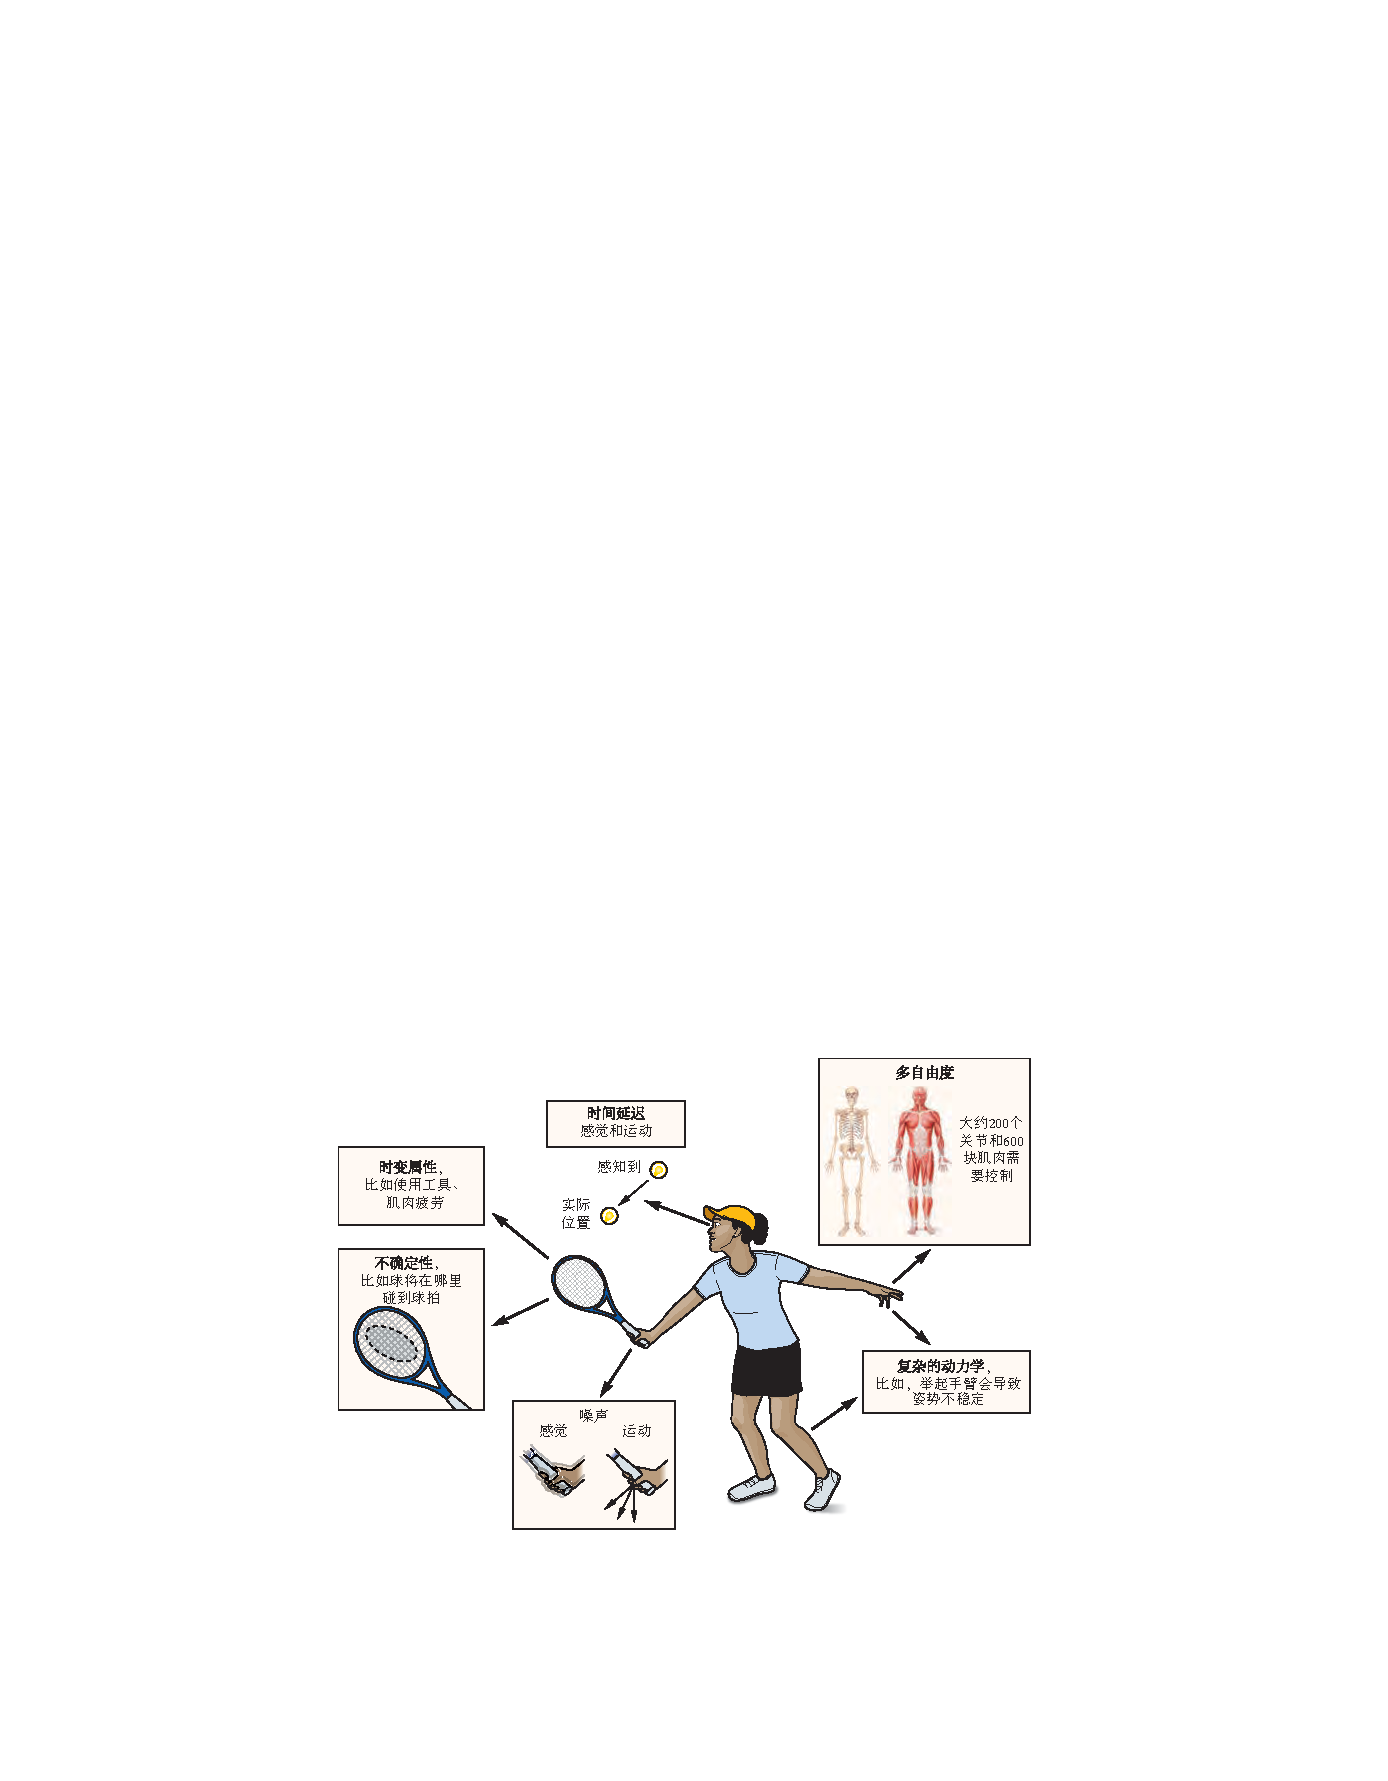
\includegraphics[width=0.82\linewidth]{chap30/fig_30_1}
	\caption{感觉运动控制的挑战。}
	\label{fig:30_1}
\end{figure}


其次,即使球员能够可靠地估计球的轨迹,她也必须根据感官信号确定她将使用 600 块肌肉中的哪块肌肉来移动她的身体和球拍来拦截球。
控制这样的系统可能具有挑战性,因为很难在具有许多自由度(例如,大量个体肌肉)的系统中有效地探索所有可能的动作,这使得学习变得困难。
我们将看到运动系统如何通过控制肌肉群(称为协同作用)来降低肌肉骨骼系统的自由度以简化控制。


第三,不需要的干扰(称为噪声)会破坏许多信号,并且存在于感觉运动控制的所有阶段,从感觉处理到计划,再到运动系统的输出。
例如,在网球发球中,即使发球者试图击中球场上的同一位置,这种噪音也会导致球落在不同的位置。
反映球位置的感官反馈和运动输出都被噪音污染了。
这种噪音中固有的可变性限制了我们准确感知和准确行动的能力。
我们的运动命令中的噪音量往往会随着命令越强(即更大的力)而增加。
这限制了我们同时快速移动和准确移动的能力,从而需要在速度和准确性之间进行权衡。
我们将看到有效的运动规划如何最大限度地减少噪音对任务成功的不利影响。


第四,时间延迟存在于感觉运动系统的所有阶段,包括受体动力学引起的延迟、沿神经纤维和突触的传导延迟,以及响应运动指令的肌肉收缩延迟。
总之,这些延迟可能在 100 毫秒的数量级,取决于特定的感觉形态(例如,视觉比本体感觉更长)和处理的复杂性(例如,面部识别比运动感知更长)。
因此,我们实际上生活在过去,控制系统只能访问关于世界和我们自己身体的过时信息。
在尝试快速移动时,此类延迟可能会导致不稳定,因为我们会尝试纠正我们察觉到但已不存在的错误。
我们将看到大脑如何预测身体和环境的未来状态,以减少此类延迟的负面影响。


第五,身体和环境在短期和长期的时间尺度上都会发生变化。
例如,在相对较短的比赛时间内,运动员必须纠正因疲劳而减弱的肌肉以及下雨时球场表面的变化。
在更长的时间尺度上,随着我们的四肢变长和体重增加,我们的运动系统的特性在生长过程中会发生巨大变化。
正如我们将看到的,运动系统不断变化的特性使我们必须高度重视利用运动学习来适当调整控制的能力。


最后,运动指令与后续动作之间的关系非常复杂。
每个身体部分的运动通过机械相互作用在所有其他身体部分产生扭矩,并可能产生运动。
例如,当一名球员举起球拍击球时,她必须预见到不稳定的力量并抵消它们以保持平衡。
事实上,当我们站立时向前举起手臂时,首先激活的肌肉是踝屈肌,以确保我们保持直立。
我们将看到感觉运动系统如何控制不同部分的运动以保持动作的精细协调。



\section{可以自愿、有节奏或反射性地控制动作}

虽然运动通常根据功能分类,如眼球运动、抓握(伸手和抓握)、姿势、运动、呼吸和说话,但其中许多功能是由重叠的肌肉群提供的。
此外,相同的肌肉群可以有意识地、有节奏地或反射性地受到控制。
例如,控制呼吸的肌肉可以用来在潜入水下之前自主地深呼吸,以有规律的吸气和呼气循环自动和有节奏地呼吸,或者对喉咙中的有害刺激做出反射性反应,产生咳嗽。


自主运动是那些在意识控制下的运动。
有节奏的运动也可以自主控制,但与自主运动的不同之处在于,它们的时间和空间组织在更大程度上由脊髓或脑干回路自主控制。
反射是由脊髓或脑干中的神经回路产生对特定刺激的刻板反应(尽管有些反射涉及通过皮层的通路)。
这些反应比自愿反应发生的时间更短。


尽管我们可能打算有意识地执行一项任务或计划一系列动作,并且有时会意识到自己决定在特定时刻移动,但动作通常似乎是自动发生的。
对运动的瞬间控制不需要有意识的过程。
我们执行最复杂的动作,而没有考虑所需的实际关节运动或肌肉收缩。
网球运动员不会有意识地决定使用哪些肌肉来反手接发球,或者必须移动哪些身体部位来拦截球。
事实上,在每个身体动作发生之前考虑它会扰乱玩家的表现。



\section{运动命令通过感觉运动过程的层次结构产生}

尽管肌肉骨骼系统的最终输出是通过脊髓中的运动神经元进行的,但肌肉对特定动作的运动控制是通过控制中心的层次结构进行的。
这种安排可以简化控制:高层可以规划更多的全局目标,而低层则关心这些目标如何实现。


在最低层次上,肌肉本身具有的特性可以在没有任何运动命令变化的情况下对控制产生影响。
与机器人的电动马达不同,肌肉具有大量的被动特性,这取决于作用在肌肉上的运动命令以及肌肉的长度和长度变化率(第~\ref{chap:chap31}~章)。
作为一个简单的近似值,肌肉可以被看作像弹簧(拉伸时增加张力,缩短时减小张力)和阻尼器(随着拉伸率的增加而增加张力)。
对于小的扰动,这些特性倾向于稳定肌肉的长度,从而稳定肌肉作用的关节。
例如,如果外部扰动使关节伸展,屈肌会被拉伸,增加张力,而伸肌会缩短,张力会降低,张力的不平衡会使关节回到原来的位置。
这种控制的一个特殊优势是:与运动层次结构中的更高层不同,这种力的变化以最小的延迟起作用,因为它们只是肌肉被动物理特性的影响。


除了肌肉的被动特性外,感觉输入可以直接引起运动输出,而无需高层脑中枢的干预。
感觉运动反应,如脊髓反射,控制局部干扰或伤害性刺激。
反射是由脊髓或脑干中的简单神经回路产生的对特定刺激的刻板反应。
例如,脊柱屈肌缩回反射可以在没有来自大脑的任何下行输入的情况下将您的手从热炉中移开。
这种反应的优点是速度快;
缺点是它们不如自愿控制系统灵活(第~\ref{chap:chap32}~章)。
同样,存在反射回路的层次结构。
最快的是单突触牵张反射,它驱动被拉伸的肌肉收缩。 
在这个反射回路中,被肌肉中的牵张感受器(肌梭)激活的感觉神经元直接突触到运动神经元上,导致同一块肌肉收缩。
从刺激到响应的时间约为 25 毫秒。
这种反射可以通过敲打髌骨正下方的股四头肌肌腱进行临床测试。


虽然这种单突触牵张反射不适用于短时间尺度,但涉及更高层结构(如运动皮层)的多突触反射可以在 70 毫秒左右产生响应。
与单突触反射不同,多突触反射可适应行为目标的变化,因为连接感觉神经元和运动神经元的回路可以通过任务相关特性进行修改。
反射的强度往往会随着肌肉中的张力而增加(称为增益缩放),因此,可以通过共同收缩关节周围的一组肌肉来放大反射,从而以更大的力响应扰动。
事实上,我们在过马路时牵着一个叛逆的孩子的手时就使用了这种共同收缩。
这种策略可以放大反应,从而减少随机外力引起的手臂偏差。


最后,自主运动是那些受大脑有意识控制的运动。
自主运动可以在没有刺激的情况下产生或用于补偿扰动。
响应物理扰动而产生自主运动的时间取决于扰动的性质(模态和大小)以及是否可以在扰动发生之前指定响应。
例如,对小物理扰动的自愿校正可能会延迟约 110 毫秒。


尽管我们已经描述了从反射到自愿控制的不同层次的运动层次之间的明显区别,但实际上,在跨越不同延迟的连续反应中,这种区别是模糊的。
增加响应时间允许额外的神经回路参与感觉运动回路,并往往会增加响应的复杂性和适应性,导致在向上提升到运动层次时需要在响应速度和处理的复杂性之间进行权衡。



\section{运动神经信号受前馈和反馈控制}

在本节中,我们将首先说明一些对处理感觉延迟、感觉噪声和运动噪声问题很重要的控制原理。
为简单起见,我们将讨论限制在相对简单的动作上,例如响应头部运动移动眼睛或将手从一个位置移动到另一个位置。
我们考虑两大类控制,前馈和反馈,它们在运动过程中对感官反馈的依赖程度不同。



\subsection{快速运动需要前馈控制}

有些动作是在没有监测动作产生的感官反馈的情况下执行的。
在这种前馈控制情况下,运动命令的生成不考虑感官后果。
因此,此类命令也称为开环,反映了感觉运动环路不是由感觉反馈完成的事实(图~\ref{fig:30_2}A)。


\begin{figure}[htbp]
	\centering
	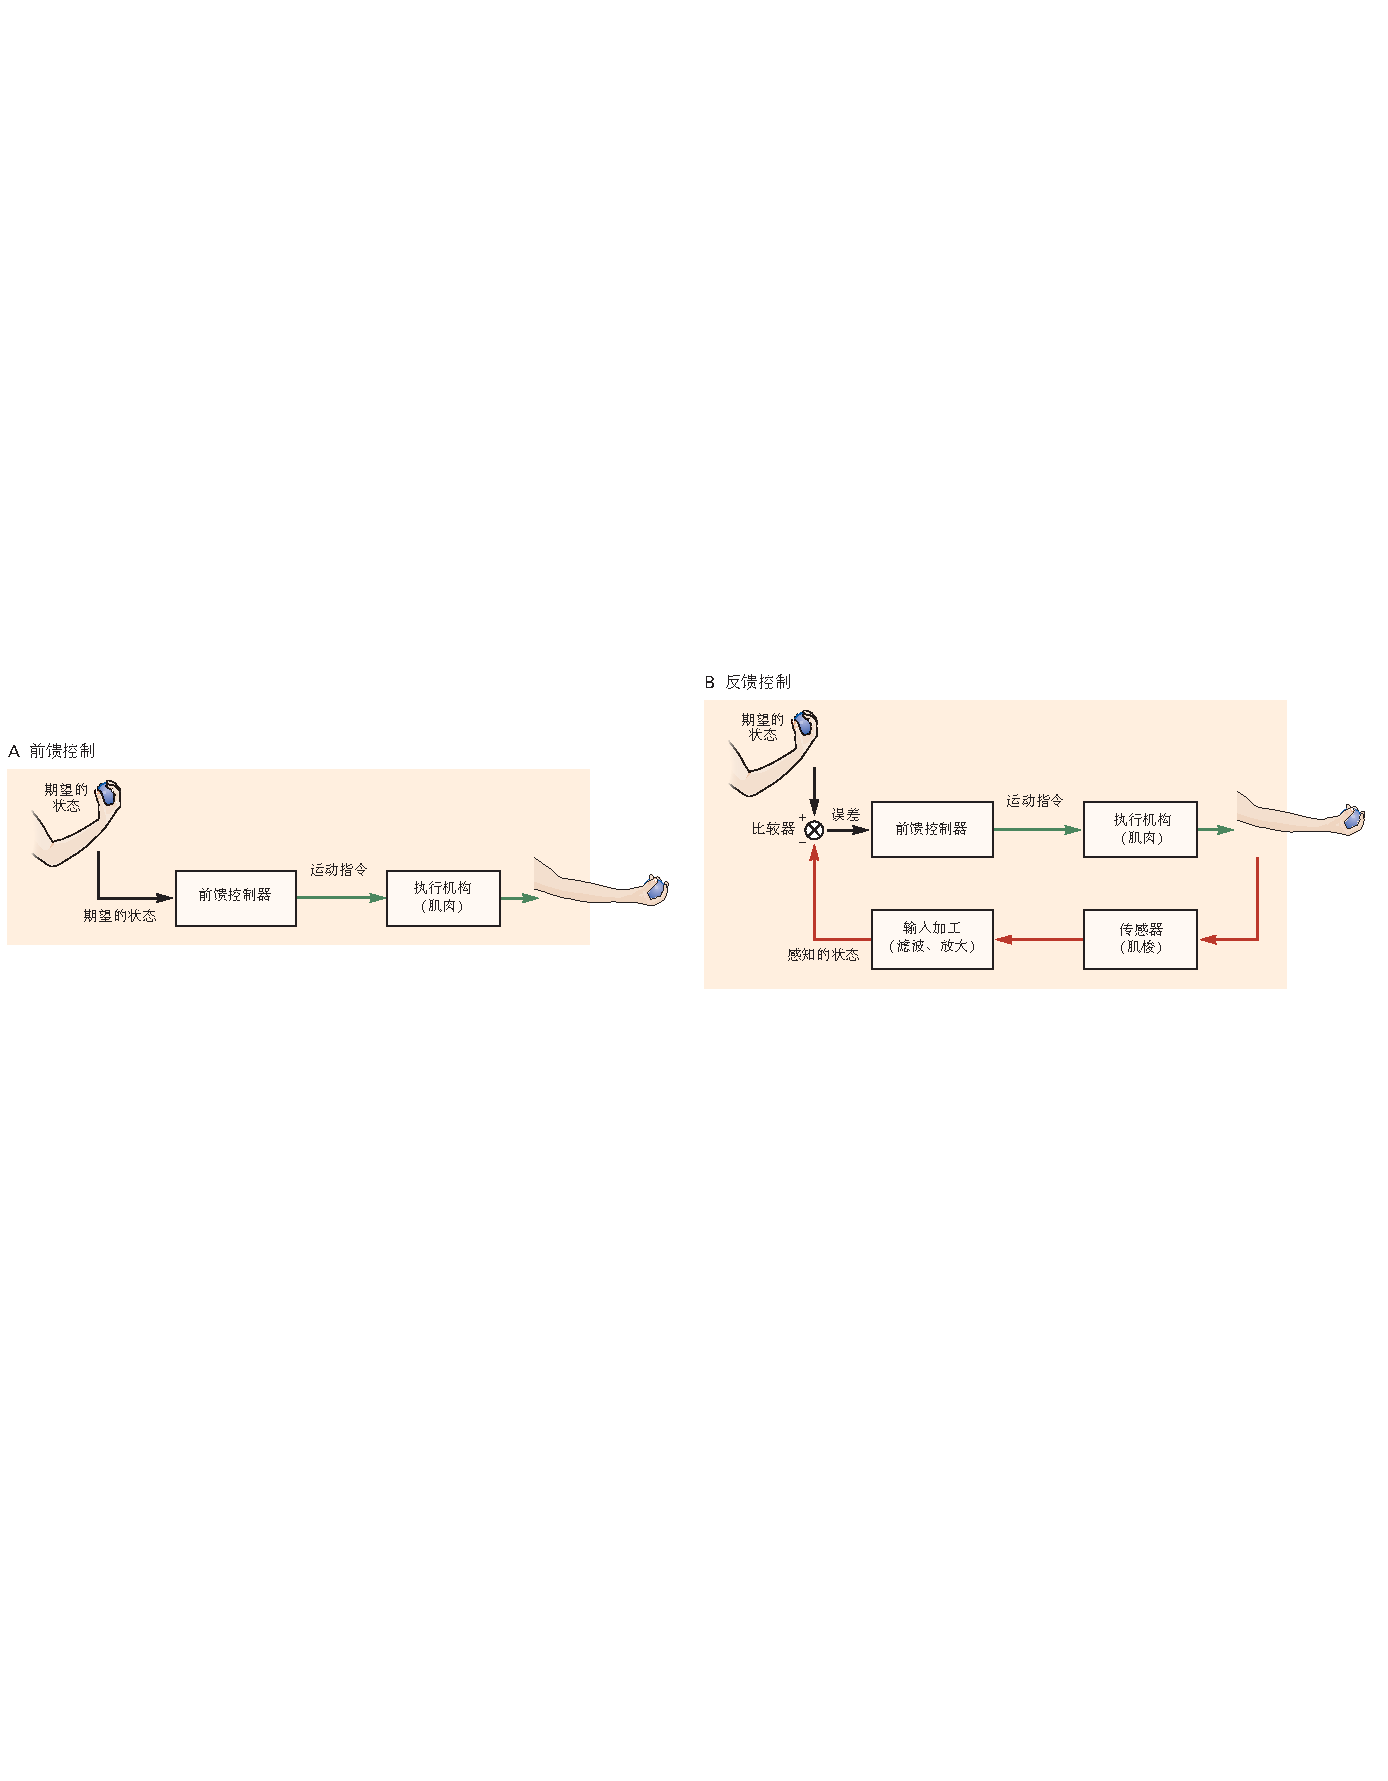
\includegraphics[width=1.0\linewidth]{chap30/fig_30_2}
	\caption{前馈和反馈控制。
		\textbf{A.} 前馈控制运动命令基于所需状态。
		不会监控移动过程中出现的错误。
		虽然我们说明了手臂前馈控制的元素,但只有任何手臂运动的初始部分是由前馈信号驱动的,并且运动通常涉及反馈控制。
		\textbf{B.} 通过反馈控制,比较所需状态和感测状态(在比较器处)以生成误差信号,这有助于形成运动命令。
		感觉信息反馈给比较器可能会有相当大的延迟。}
	\label{fig:30_2}
\end{figure}


开环控制需要一些关于身体的信息,以便生成适当的命令。
例如,它应该包括有关运动系统动力学的信息。
这里的“动力学”是指施加的运动命令(或扭矩或力)与随后的身体运动(例如关节旋转)之间的关系。
对于完美的开环控制,需要反转动力学以计算将产生所需运动的运动命令。
执行这种反转的神经机制称为逆向模型,是一种内部模型(方框~\ref{box:30_1})。
耦合到开环控制的逆模型可以确定需要哪些运动命令来产生实现目标所需的特定运动。


\begin{proposition}[内部模型] \label{box:30_1}
	
	\quad \quad 数值模型在物理科学中的应用有着悠久的历史。
	数值模型是复杂物理系统的抽象定量表示。
	有些从表示初始条件的方程和参数开始,在时间或空间上向前运行,以在未来的某个状态下生成物理变量。
	例如,我们可以构建一个天气模型,预测两周后的风速和温度。
	
	\quad \quad 其他模型从一个状态开始,一组具有特定值的物理变量,并以相反的方向运行,以确定系统中的哪些参数解释了该状态。
	当我们将一条直线拟合到一组数据点时,我们正在构建一个逆模型,该模型基于线性系统的方程来估计斜率和截距。
	因此,反向模型可以允许我们知道如何设置系统的参数以获得期望的结果。
	
	\quad \quad 在过去的50年里,神经系统有类似的物理世界预测模型来指导行为的想法已经成为神经科学的一个主要问题。
	这种模型被称为“内部”,因为它是在神经回路中实例化的,因此是中枢神经系统的内部。
	这个想法起源于\textit{肯尼思$\cdot$克雷克}关于认知功能内部模型的概念。
	在他1943年出版的《解释的本质》一书中,克雷克可能是第一个提出生物体利用外部世界的内部表征的人:
	
	\quad \quad 如果生物体的头脑中有一个外部现实和自身可能行动的“小规模模型”,它就能够尝试各种替代方案,得出哪种方案最好,在未来情况出现之前对其做出反应,利用过去事件的知识来应对现在和未来,并以各种方式做出更全面、更安全、以及以更有效的方式应对面临的紧急情况。
	
	\quad \quad 在这种观点中,内部模型允许生物体在考虑潜在行动的后果,但无需实际投入这些行为。
	在感觉运动控制的背景下,内部模型可以回答两个基本问题。
	首先,我们如何生成作用于肌肉的运动命令,从而控制我们身体的行为?
	第二,我们如何预测我们自己的运动指令的后果?
	
	\quad \quad 中枢神经系统必须同时进行控制和预测,才能获得熟练的运动表现。
	预测和控制是一枚硬币的两面,这两个过程精确地映射到正向和反向模型上(图~\ref{fig:30_3})。
	预测将运动指令转化为预期的感觉结果,而控制将期望的感觉结果转化为运动指令。
	
\end{proposition}


尽管不监控行动的后果似乎适得其反,但有充分的理由不这样做。
如前所述,主要原因是感知和行动都有延迟。
也就是说,感觉受体将刺激转化为神经信号并将这些信号传送到中枢神经元需要时间。
例如,视觉输入可能需要大约 60 毫秒才能在视网膜中处理并传输到视觉皮层。
除了传入感觉系统的延迟外,中央处理、传出信号向运动神经元的传输以及肌肉的反应也存在延迟。
总之,组合的感觉运动回路延迟是可观的,对于视觉刺激的运动反应大约为 120 到 150 毫秒。
这种延迟意味着像扫视这样在 30 毫秒内重定向凝视的运动不能使用感官反馈来引导运动。
即使对于较慢运动,比如要时500毫秒的伸手,也不能使用感官信息指导运动的初始部分,因此必须使用开环控制。


开环控制也有缺点。
任何因计划或执行不准确而导致的运动错误都不会得到纠正,因此会随着时间或连续运动而复合。
受控系统越复杂,通过学习得到准确的逆模型就越困难。


纯开环控制系统的一个例子是响应头部旋转的眼睛控制。
\textit{前庭-眼动反射}(第~\ref{chap:chap27}~章)使用开环控制在头部旋转期间将视线固定在物体上。
前庭迷路感知头部旋转并通过三突触回路驱动眼睛的适当运动。
反射在运动过程中不需要(或使用)视觉(在黑暗中转动头部时眼睛保持稳定的注视)。
来自前庭系统的感觉信息确实会驱动眼球运动,但控制是前馈的(在运动过程中不会纠正出现的任何错误)。
这种精确的开环控制是可能的,因为眼睛的动态特性相对简单,前庭迷路可以直接感知头部的旋转,并且眼睛往往不会受到外部事件的显著干扰。
相比之下,为复杂的肌肉骨骼系统(例如手臂)优化逆模型非常困难,因此,手臂运动的控制需要某种形式的误差校正。



\subsection{反馈控制使用感官信号来纠正动作}

为了纠正出现的运动错误,必须监测运动。
执行纠错的系统被称为反馈或闭环控制,因为感觉运动回路是完整的(图~\ref{fig:30_2}B)。


最简单的反馈控制形式是当误差超过某个阈值时控制系统产生固定响应。
在大多数中央供暖系统中都可以看到这样的系统,其中恒温器被设置为所需的温度。
当房屋温度低于指定水平时,加热会打开,直到温度达到该水平。
虽然这样的系统简单且有效,但它的缺点是输入房屋的热量与实际温度和所需温度之间的差异(误差)无关。
更好的系统是控制信号与误差成正比的系统。


这种运动的比例控制包括感知手的实际位置和期望位置之间的误差。
校正运动命令的大小与误差的大小成比例并且在减小误差的方向上。
每单位位置误差校正运动命令增加或减少的量称为增益。
通过不断纠正运动,反馈控制对感觉运动系统中的噪声和环境扰动都具有鲁棒性。


虽然反馈控制可以更新命令以响应运动期间出现的偏差,但它对反馈延迟很敏感。
在没有任何延迟的情况下,随着反馈控制器增益的增加,系统将以更高的保真度跟踪所需位置(图 30–4)。
然而,随着反馈延迟的增加,控制系统可能开始振荡并最终变得不稳定。
这是因为随着延迟,系统可能会响应不再存在的错误,甚至可能在错误的方向上进行纠正。


\begin{figure}[htbp]
	\centering
	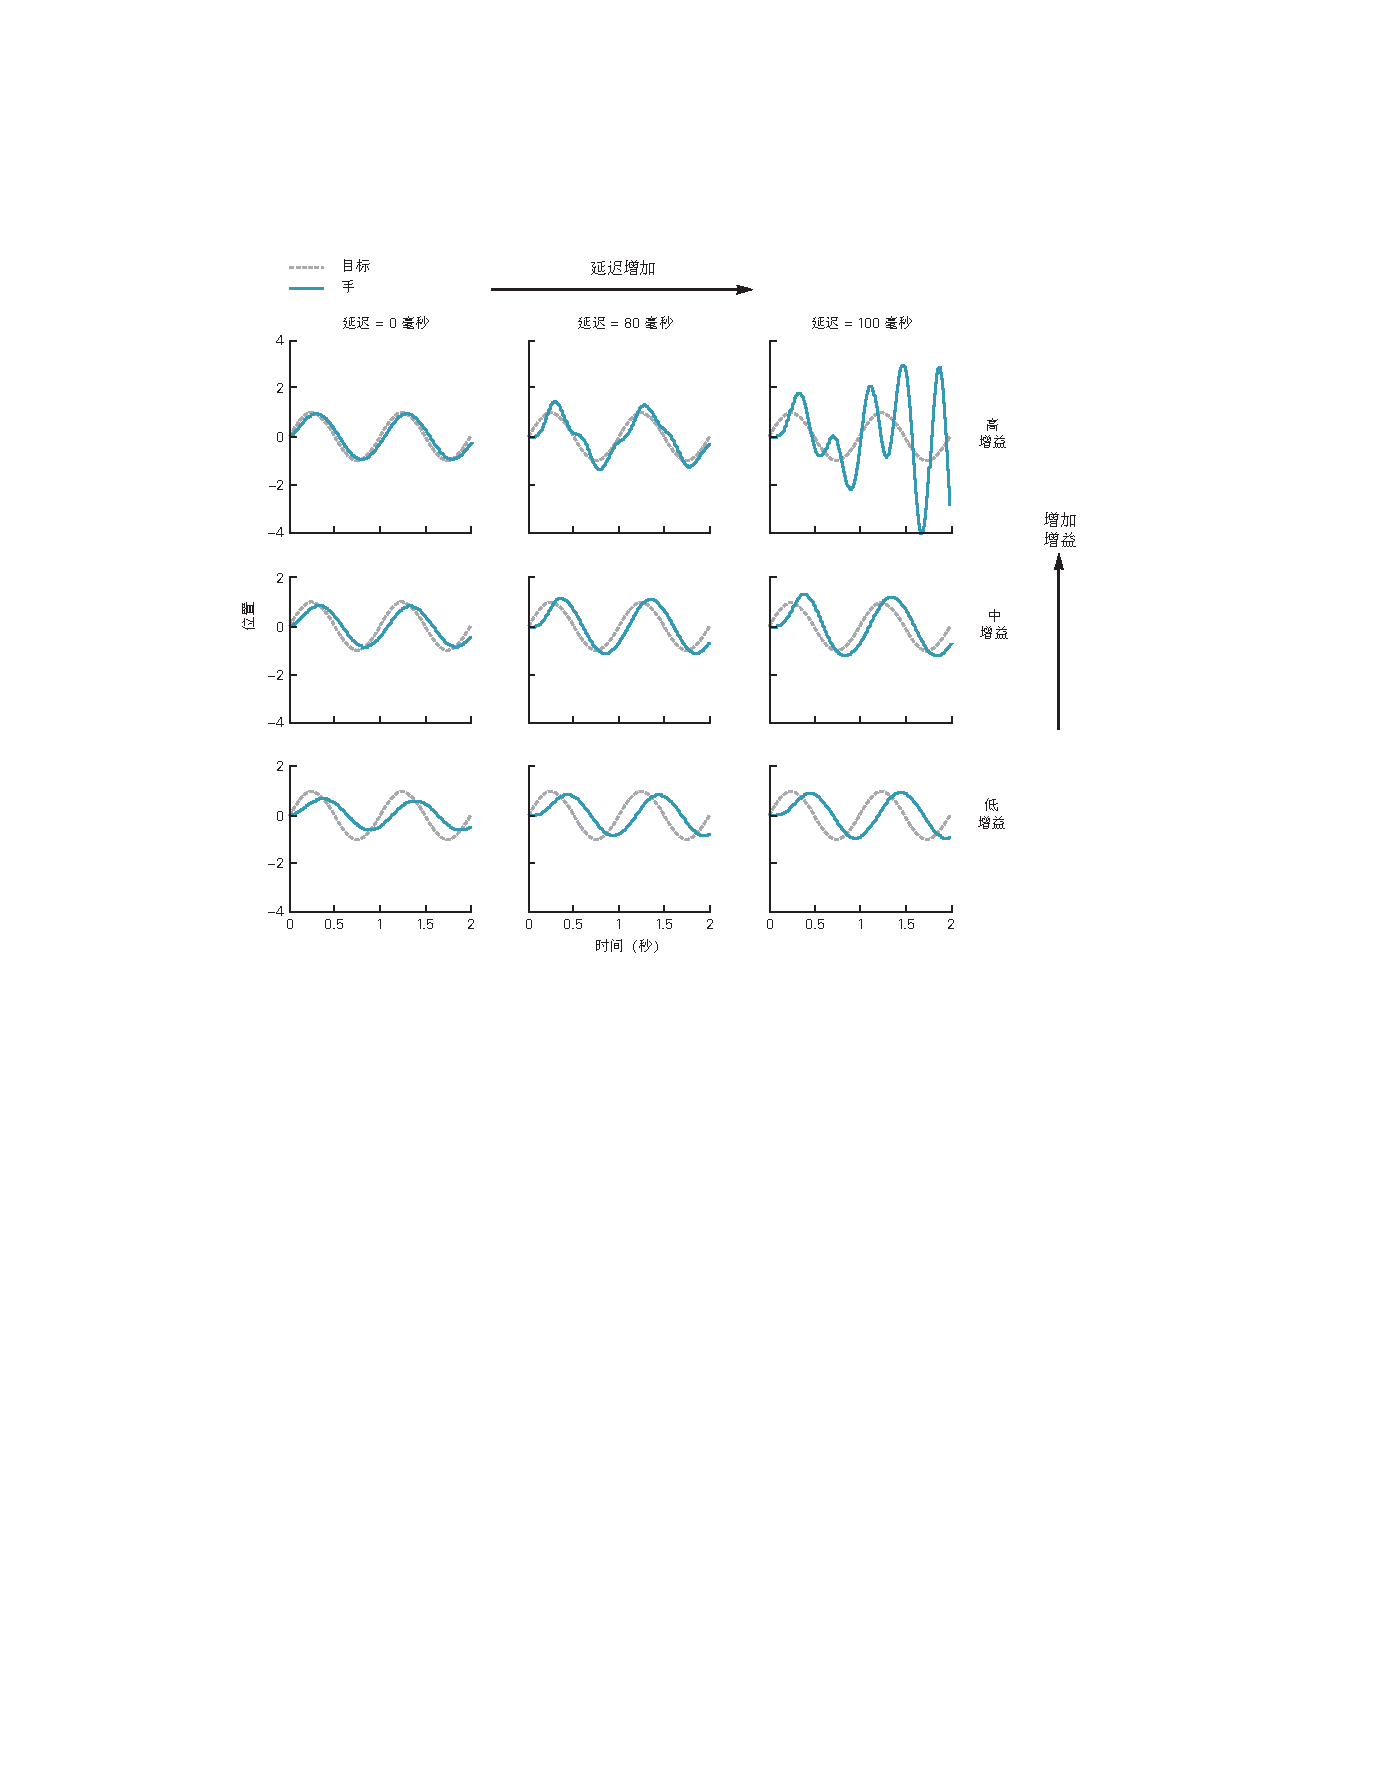
\includegraphics[width=0.9\linewidth]{chap30/fig_30_4}
	\caption{反馈控制中增益和延迟的相互作用。
		反馈控制器尝试跟踪一维正弦运动目标的性能。
		传达位置误差的传感反馈信号在一段时间(延迟)后到达,运动系统尝试通过增加或减小相对于误差的命令大小(增益)来纠正误差。
		该图显示了错误瞬时反馈(无延迟)(左列)或延迟 80 或 100 毫秒(中列和右列)的性能。
		当增益高且延迟低时,跟踪效果非常好。
		但是,当延迟增加时,由于控制器正在补偿 80 或 100 毫秒之前存在的误差,因此校正可能不适用于当前误差。
		可以降低增益以保持稳定性,但由于反馈控制器只能缓慢地纠正错误,因此跟踪变得不准确。
		在低增益(底行)时,反馈控制器只能缓慢地纠正错误,并且跟踪不准确。
		随着增益增加(中间行),反馈控制器纠正错误的速度更快,跟踪性能也得到改善。
		在高增益(顶行)下,系统校正速度很快,但容易过度校正,当反馈时间延迟达到生理时间延迟(右上)数量级时,会导致不稳定。
		由于控制器正在补偿 100 毫秒前存在的误差,因此校正可能不适用于当前误差。
		这种过度校正会导致振荡,并且是一种解释神经系统疾病中出现的某些形式的振荡性震颤的机制。}
	\label{fig:30_4}
\end{figure}


用于跟踪移动物体的\textit{平滑跟踪}眼球运动是主要由反馈驱动的运动的一个例子。
\textit{平滑跟踪}使用反馈来最小化视网膜上的速度误差(凝视速度和目标速度之间的差异)。
我们可以比较前馈和反馈控制在最小化误差方面的效率。
比较在快速来回转动头部时注视伸出的固定手指与在头部保持静止时快速左右正弦移动手指时尝试跟踪手指的难易程度。
虽然手指与头部的相对运动在两种情况下相同,但前者是精确的,因为它使用\textit{前庭-眼动反射},而后者使用反馈(需要速度误差来驱动眼球运动),因此不太精确 ,特别是运动频率增加时。


在大多数运动系统中,运动控制是通过前馈和反馈过程的组合实现的。
稍后我们将看到这两个组成部分自然地出现在一个统一的机芯生产模型中。



\subsection{对身体当前状态的估计依赖于感觉信号和运动信号}

准确控制运动需要有关我们身体当前状态的信息,例如,身体不同部位的位置和速度。
要抓住一个物体,我们不仅需要知道物体的位置、形状和表面特性,还需要知道我们手臂和手指的当前配置,以便适当地塑造和定位手。


估计身体的状态不是一个小问题。
首先,正如我们所见,感觉信号由于感觉转导和传导时间而延迟。
因此,来自我们的肌肉、关节和视觉的信号在到达中枢神经系统时都已经过时了。
其次,我们接收到的感觉信号通常是不精确的,并且会被神经噪声破坏。
例如,如果您用一只手的手指触摸桌子的底部,并尝试用另一只手估计它在桌子顶部的位置,您可能会偏离相当大的距离。
第三,我们通常没有直接传达相关信息的传感器。
例如,虽然我们有报告肌肉长度和关节角度的传感器,但我们在肢体中没有直接确定手在空间中的位置的传感器。
因此,需要复杂的计算来尽可能准确地估计当前的身体状态。
关于大脑如何估计状态的几个原则已经出现。


首先,状态估计依赖于感觉运动转换的内部模型。
鉴于我们肢体的固定长度,手臂的肌肉长度或关节角度与手在空间中的位置之间存在数学关系。
这种关系的神经表示允许中枢神经系统在知道关节角度和节段长度的情况下估计手的位置。
计算此类感觉运动转换的神经回路就是内部模型的示例(方框~\ref{box:30_1})。


其次,可以通过组合多种感官方式来改进状态估计。
例如,关于我们四肢状态的信息来自肌梭、皮肤拉伸和手臂视觉的本体感受信息。
这些模态具有与之相关的不同量的可变性(或噪声),正如我们对一组实验数据进行平均以减少测量误差一样,可以组合这些感官模态以减少状态估计中的总体不确定性。


结合这些来源的最佳方式是让更高层的大脑中心考虑到每种模式的不确定性,并依赖于更确定的模式。
例如,手的位置可以通过本体感觉和视觉来感知。
在估计沿方位角(右-左)的位置时,手在你面前的视线往往比本体感觉更可靠,但在深度(前-后)方面则不太可靠。
因此,在估计手的方位角位置时,视觉输入应比本体感受输入具有更大的权重,反之亦然。
通过测量单独使用时每种模态的精度,可以预测同时使用两种模态时提高的精度。
实验表明,这个过程通常接近最佳。
还可以通过使用贝叶斯推理的数学将先验知识与感官输入相结合来提高精度(方框~\ref{box:30_2})。


\begin{proposition}[贝叶斯推断] \label{box:30_2}
	
	\quad \quad 贝叶斯推理是一种基于不确定信息对世界进行估计的数学框架。
	其基本思想是,概率(在0和1之间)可以用来表示对不同选择的信任程度,例如相信你用公平骰子掷六分的几率是1/6。
	
	\quad \quad 贝叶斯推理的美妙之处在于,通过使用概率规则,我们可以根据我们的经验和来自感官输入的新信息来指定信念应该如何形成和更新。
	例如,当打网球时,我们想估计球会落在哪里。
	由于视觉不能提供关于球在飞行中的位置和速度的完美信息,因此着陆位置存在不确定性。
	然而,如果我们知道我们的感觉系统中的噪声水平,那么当前的感觉输入可以用于计算不同潜在着陆位置的特定感觉输入的可能性(即概率)。
	
	\quad \quad 我们可以从反复的比赛经验中学到更多的信息:球落在球场上的位置不太可能。
	例如,反弹位置可能集中在最难回球的边界线附近。
	这种分布被称为先验分布。
	
	\quad \quad 贝叶斯规则定义了如何结合先验和似然性来对反弹位置进行最佳估计。
	虽然贝叶斯方法最初是在统计学中发展起来的,但它现在提供了一个统一的框架来理解大脑如何处理感知、运动和认知领域的不确定性。
	
\end{proposition}


第三,运动指令也可以提供有价值的信息。
如果身体的当前状态和下行运动命令都已知,则可以估计身体的下一个状态。
该估计可以从表示行为及其后果之间因果关系的内部模型中得出。
这被称为前向模型,因为它根据运动输出估计未来的感觉输入(方框~\ref{box:30_1})。
因此,正向模型可用于预测运动系统的状态将如何因运动指令而发生变化。
下行运动命令的副本被传递到前向模型中,该模型充当在环境中移动的肌肉骨骼系统的神经模拟器。
运动命令的此副本称为\textit{传出副本}(或\textit{伴随发送})。
如果我们将两者串联起来,可以更好地理解正向和反向模型。
如果每个模型的结构和参数值都是正确的,正向模型的输出(预测的行为)将与逆向模型的输入(期望的行为)相同(图~\ref{fig:30_3})。


\begin{figure}[htbp]
	\centering
	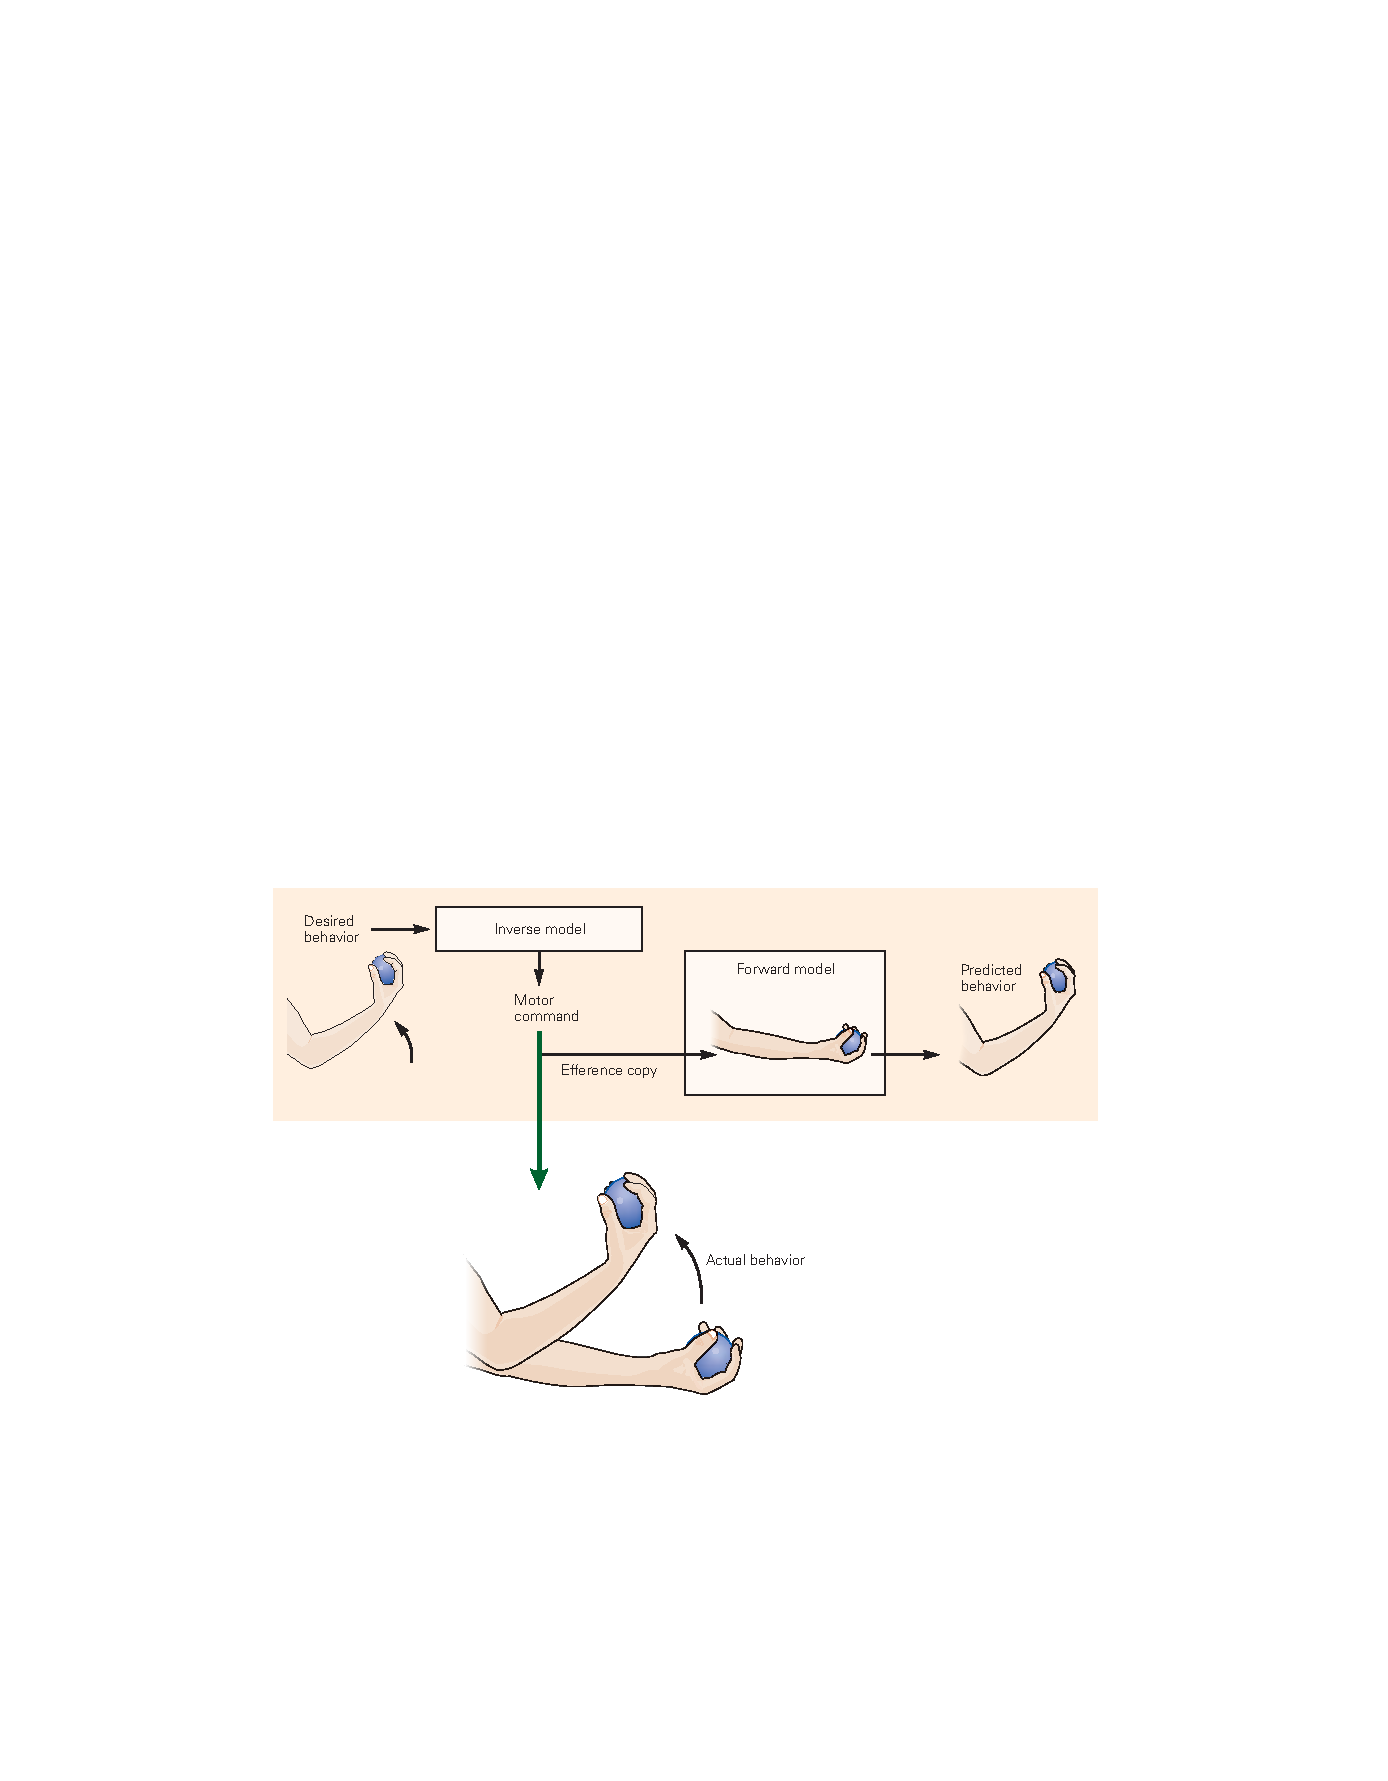
\includegraphics[width=0.93\linewidth]{chap30/fig_30_3}
	\caption{内部感觉运动模型代表身体与外部世界的关系。
		逆模型确定将产生行为目标的运动命令,例如在握球时举起手臂。
		下行运动命令作用于肌肉骨骼系统以产生运动。
		运动命令的副本被传递到前向模型,该模型模拟运动系统与世界的相互作用,从而可以预测行为。
		如果正向和反向模型都是准确的,则正向模型的输出(预测行为)将与反向模型的输入(期望行为)相同。}
	\label{fig:30_3}
\end{figure}


使用运动命令来估计身体状态是有利的,因为与延迟的感觉信息不同,运动命令在作用于肌肉骨骼系统之前可用,因此可用于预测状态的变化。
然而,如果正向模型不完全准确,则此估计会随着时间的推移而漂移,因此,感官反馈用于纠正状态估计,尽管它有延迟。


运动命令用于状态估计似乎令人惊讶。
事实上,正向模型的第一个演示使用了一个仅依靠运动命令来估计状态的运动系统,即眼睛在眼眶内的位置。
亥姆霍兹在试图理解我们如何定位视觉目标时首先考虑了运动预测的概念。
要计算物体相对于头部的位置,中枢神经系统必须知道物体在视网膜上的位置和眼睛的注视方向。
\textit{亥姆霍兹}的巧妙建议是,大脑不是感知注视方向,而是根据对眼部肌肉的运动命令的副本来预测它。


亥姆霍兹在自己身上做了一个简单的实验来证明这一点。
如果您在不使用眼部肌肉的情况下移动自己的眼睛(遮住一只眼睛并用手指通过眼睑轻轻按压在睁开的眼睛上),视觉目标的视网膜位置就会发生变化。
因为需要眼部肌肉的运动命令来更新眼睛状态的估计,所以预测的眼睛位置不会更新。
然而,由于视网膜图像发生了变化,这导致了世界一定已经移动的错误感知。
一个更具戏剧性的例子是,如果眼部肌肉因箭毒而暂时麻痹,那么试图移动眼睛会导致一种世界在移动的感觉。
这是因为该命令导致眼睛移动的状态估计,但是在固定的视网膜输入(由于麻痹)的情况下,唯一一致的解释是世界已经移动。


最后,最好的状态估计是通过将感觉方式与运动命令相结合来实现的。
仅使用感觉反馈或仅使用运动预测的缺点可以通过监视两者并使用前向模型估计当前状态来改善。
执行此操作的神经装置被称为观察者模型。
观察者模型的主要目标是补偿感觉运动延迟并减少由感觉和运动信号中的噪声引起的当前状态估计的不确定性(图~\ref{fig:30_5})。
这种模型得到了关于神经系统如何估计手部位置、姿势和头部方向的实证研究的支持。
我们将看到如何使用此类模型来解码脑机接口中的神经信号(第~\ref{chap:chap39}~章)。


\begin{figure}[htbp]
	\centering
	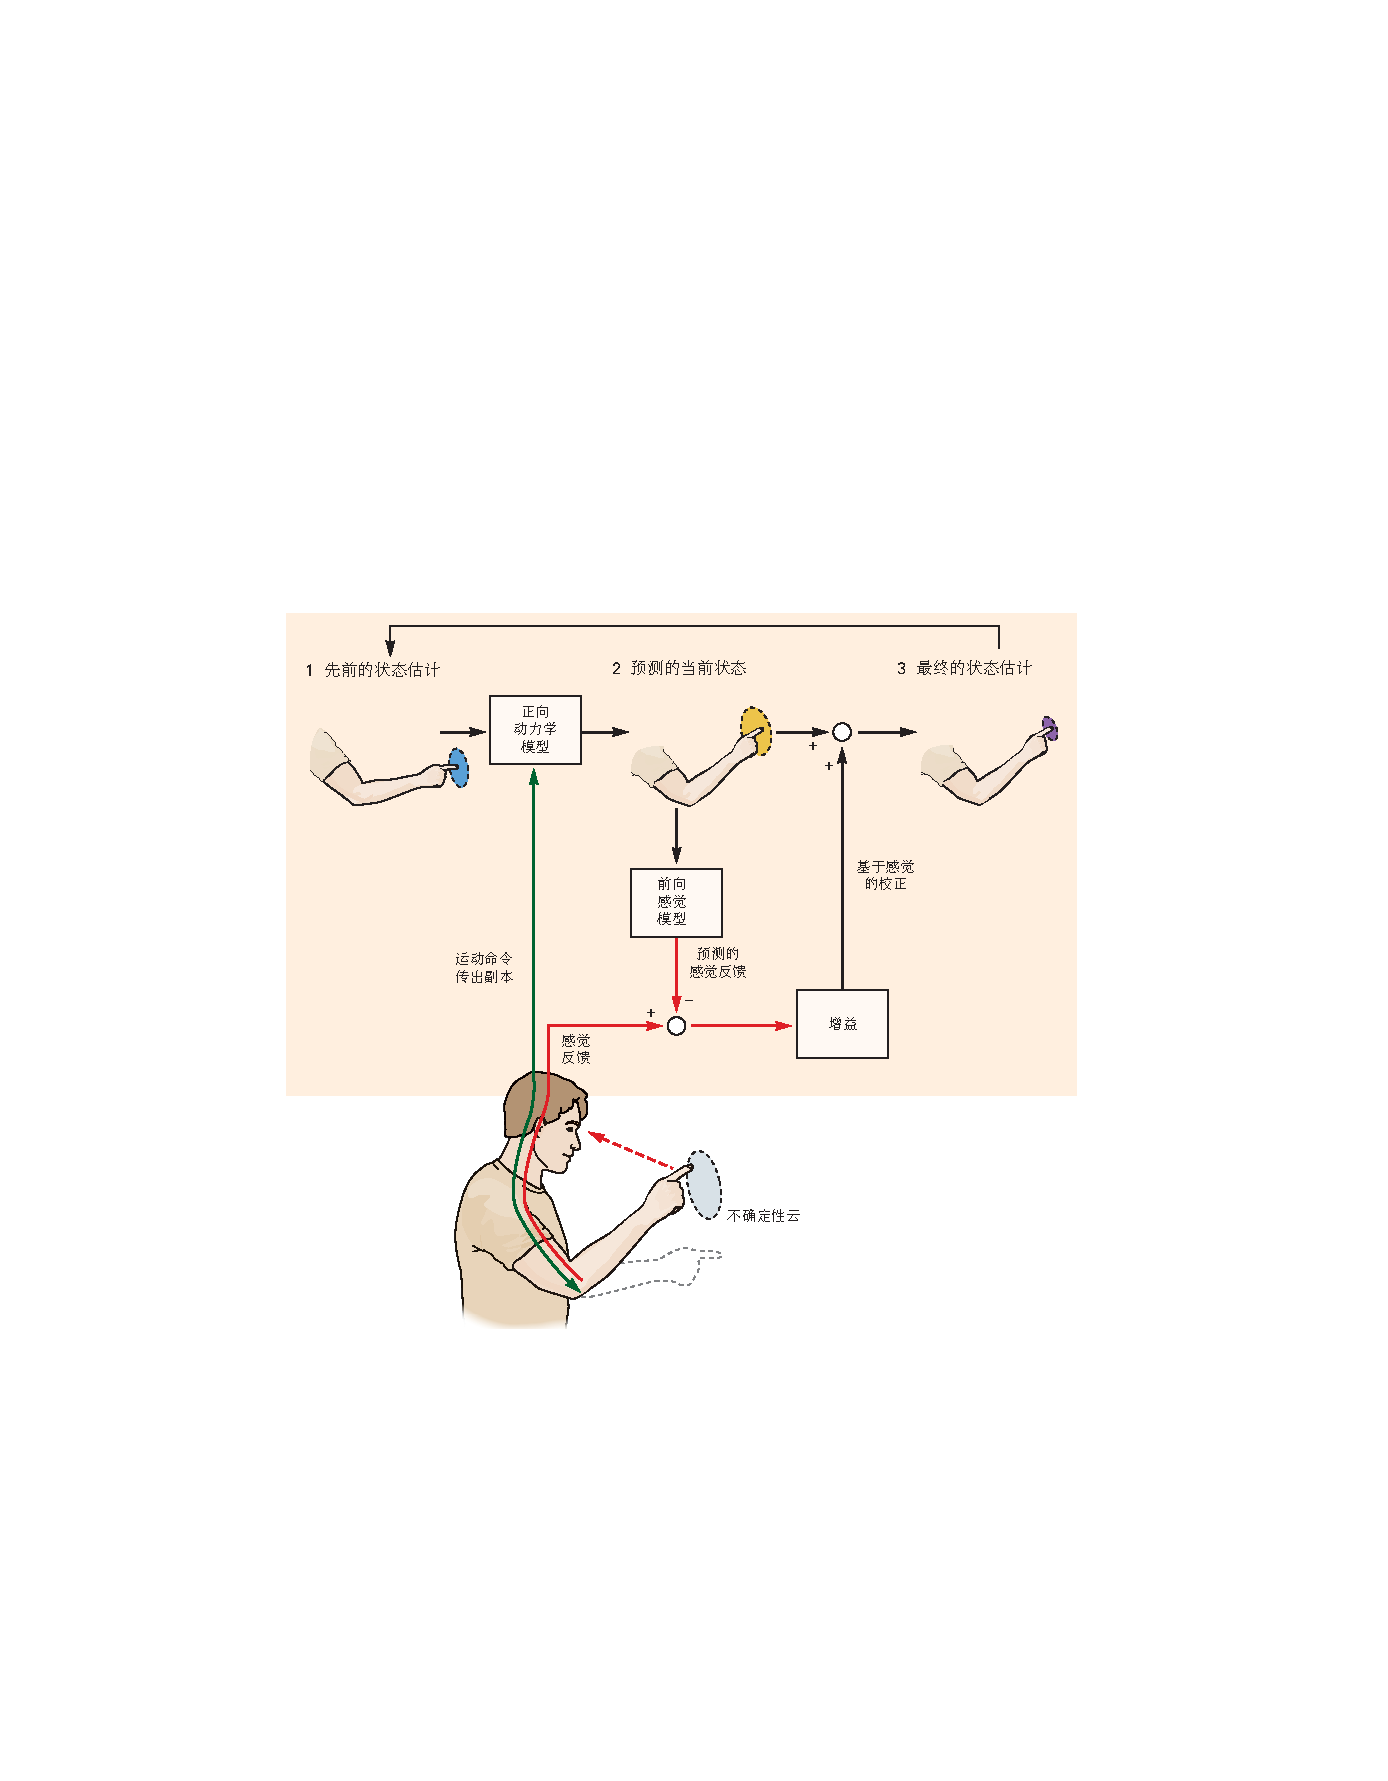
\includegraphics[width=0.9\linewidth]{chap30/fig_30_5}
	\caption{观察者模型。
		该模型用于估计手指在手臂运动期间的位置。
		使用运动命令的影响副本和动力学的前向模型更新(2,黄色云)可能的手指位置分布的先前估计(1,蓝色云)。
		手指位置的更新分布大于先前估计的分布。
		然后,该模型使用前向感觉模型来预测这些新手指位置会发生的感觉反馈,并使用预测和实际感觉反馈之间的误差来校正当前手指位置的估计。
		这种校正将感觉错误转变为状态错误,并且还确定了对效果复制和感觉反馈的相对依赖。
		当前手指位置(3,紫云)的最终估计具有较少的不确定性。
		由于此序列重复多次,此估计将成为后续移动的新的先前估计。
		为清楚起见,图中省略了必须补偿的感官反馈延迟。}
	\label{fig:30_5}
\end{figure}


状态估计不是一个被动的过程。
熟练的表现需要有效和高效地收集和处理与动作相关的感官信息。
感官信息的质量取决于我们的行为,因为我们看到、听到和触摸到的东西都会受到我们的动作的影响。
例如,眼球运动系统通过将中央凹定位到视觉场景中的兴趣点来控制眼睛的感觉输入。
因此,运动可用于有效地收集信息,这一过程称为主动感知。
主动感知涉及两个主要过程:感知,我们通过它处理感官信息并对世界做出推断,以及行动,通过它我们选择如何对世界进行采样以获得有用的感官信息。
眼球运动可以揭示熟练表演者和业余表演者之间的区别。
例如,板球比赛中的击球手会预测性扫视到他投出的球会落地的地方,等待它弹起,并在弹起后用追逐眼球的运动来追踪球的轨迹。
第一次扫视的较短延迟将专家与业余击球手区分开来。
因此,运动系统也可用于改善我们对世界的感知,从而收集信息,进而帮助我们实现运动目标。



\subsection{预测可以补偿感觉运动延迟}

正如我们所见,反馈延迟会导致运动过程中出现问题,因为延迟的信息不能反映身体和世界的当前状态。
间歇性和预测这两种策略可以补偿这种延迟,从而提高运动过程中信息的准确性。
间歇性运动会暂时被休息打断,如眼球扫视和手动跟踪。
如果休息间隔大于感觉运动回路的时间延迟,间歇性会促进更准确的感觉反馈。
预测是一种更好的策略,正如我们所见,它可以构成状态估计器的主要组成部分。


神经系统使用不同的控制模式,这些模式在不同程度上依赖于预测和感觉反馈。
不同条件下目标操作的差异很好地说明了这些模式。
当物体的行为不可预测时,感官反馈为估计负载提供了最有用的信号。
例如,在放风筝时,我们需要几乎不断地调整抓地力以应对不可预知的风流。 
在处理这种不可预测性时,抓力需要很大以防止打滑,因为抓力的调整往往滞后于负载力的变化(图~\ref{fig:30_6}A)。


\begin{figure}[htbp]
	\centering
	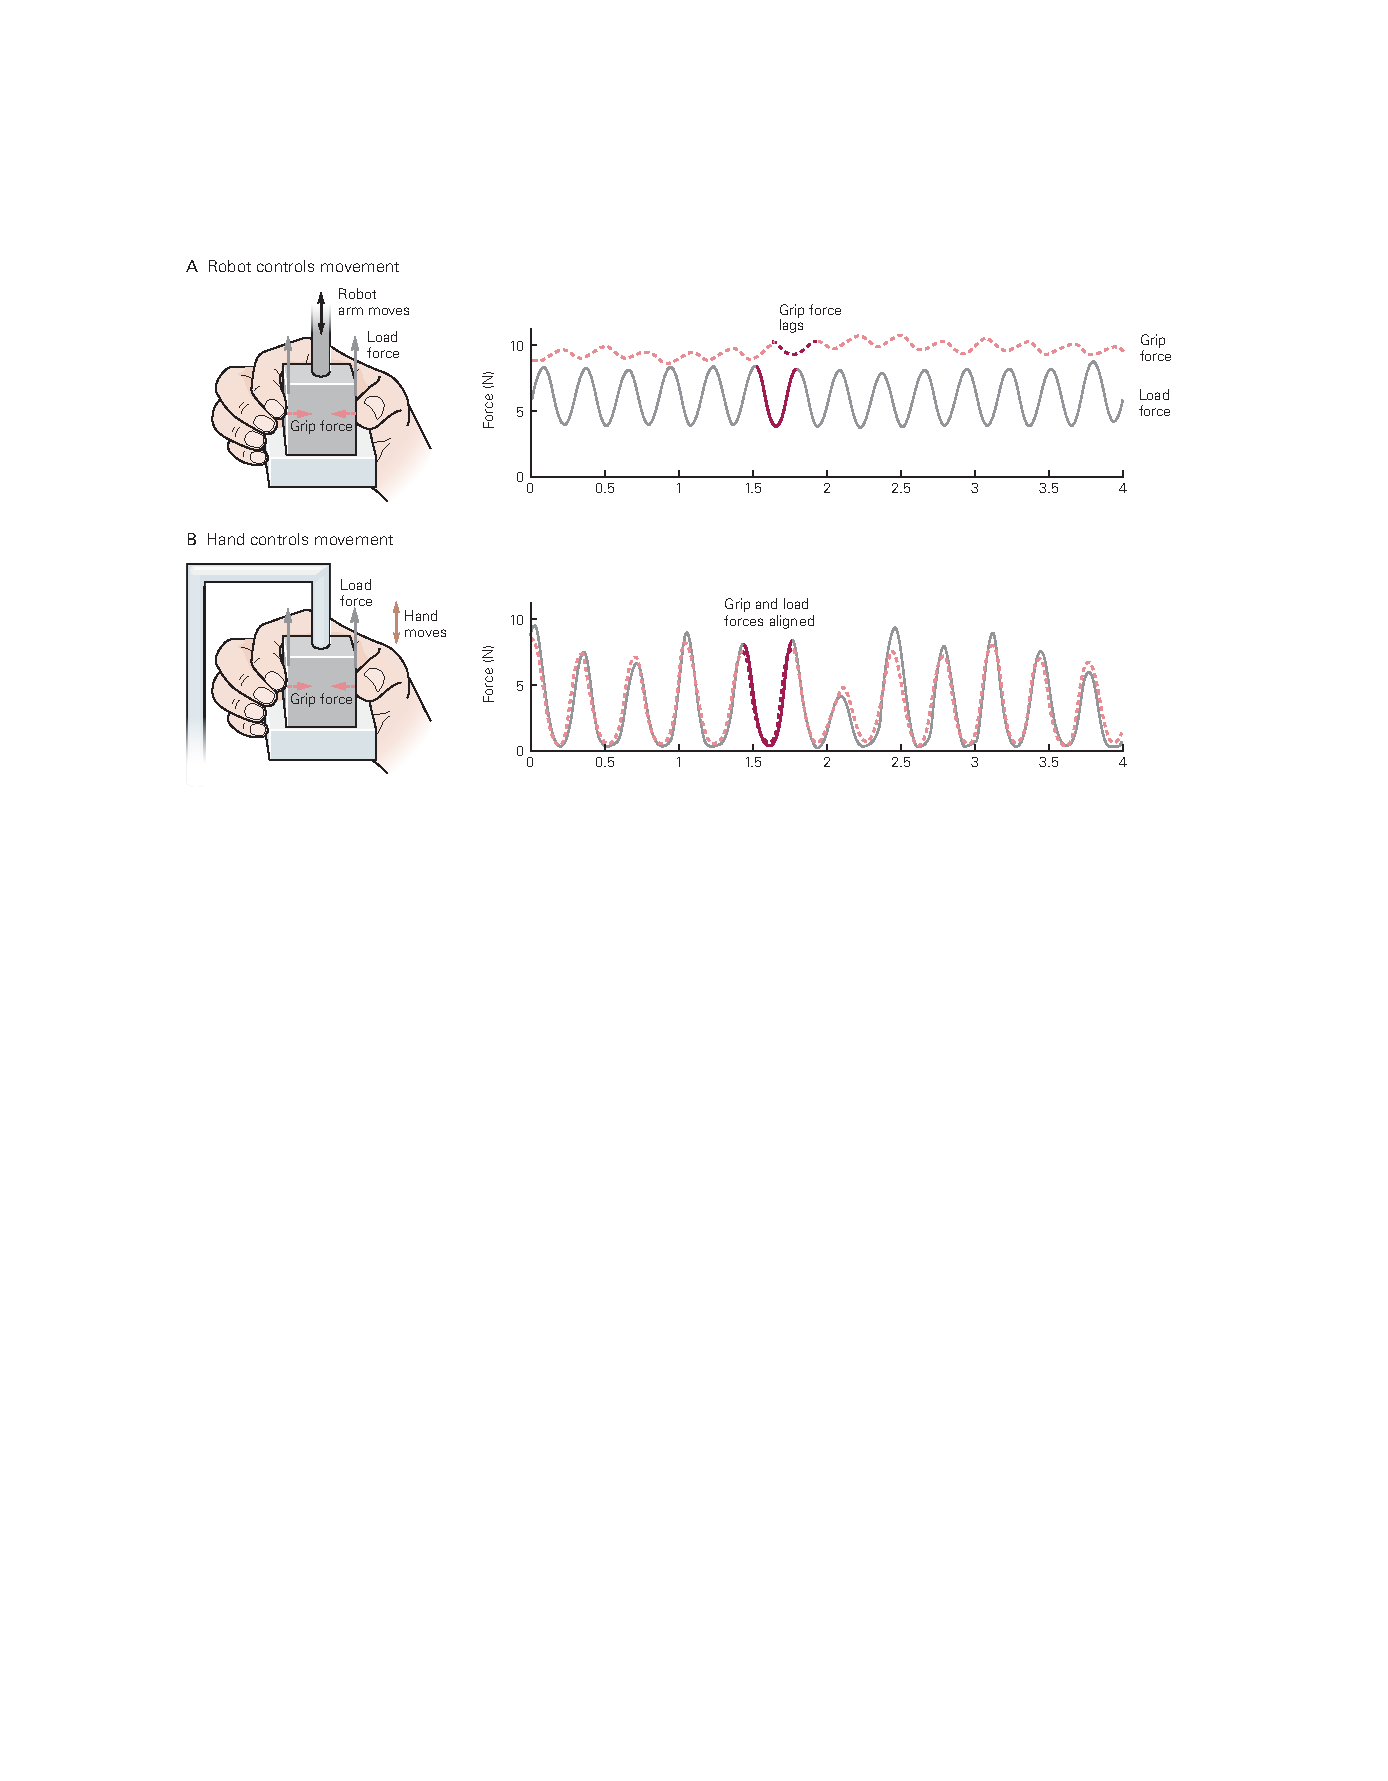
\includegraphics[width=1.0\linewidth]{chap30/fig_30_6}
	\caption{对自发动作的预期控制\cite{blakemore1998predicting}。
		\textbf{A.} 当受试者被指示保持机械地施加正弦负载力的物体时,手指的握力高以防止滑动,并且握力调制滞后于负载力的变化。
		这对于导致相应握力(暗红色虚线)的负载力调制的一部分(暗红色实线)来说是突出显示的,该握力被延迟。(试验持续时间4秒)。
		\textbf{B.} 当受试者通过下拉固定物体产生类似的负载曲线时,可以预期负载力,因此,握力较低并且也跟踪负载力而没有延迟。}
	\label{fig:30_6}
\end{figure}


然而,当处理具有稳定属性的目标时,预测控制机制会很有效。
例如,当负载因自身产生的动作(例如移动手臂)而增加时,握力会随负载力瞬间增加(图~\ref{fig:30_6} B)。
负载的感官检测速度太慢,无法解释握力的这种快速增加。


这种预测控制对于灵巧行为中常见的快速运动至关重要。 事实上,这种预测能力可以通过“服务员任务”轻松证明。 
伸出一只手臂,将一本厚重的书放在手掌上。
如果您随后用另一只手取书(就像服务员从托盘中取东西),支撑手保持静止。
这表明我们有能力预测由我们自己的行为引起的负荷变化,从而在肌肉活动中产生适当且精确的定时变化。
相比之下,如果其他人从你手中拿走书,即使你在注视着拿走的过程,也几乎不可能让手保持静止。
我们将看到小脑病变如何影响这种预测能力,从而导致缺乏这种协调反应(第~\ref{chap:chap37}~章)。


检测预测和实际感官反馈之间的任何差异在运动控制中也很重要。
这种差异称为感官预测误差,可以驱动内部模型的学习,也可以用于控制。
例如,当我们拿起一个物体时,我们预计该物体何时会离开表面。
大脑对意外事件的发生或预期事件的未发生(即感觉预测错误)特别敏感。
因此,如果物体比预期更轻或更重,因此过早升起或无法升起,则会启动反应性响应。


除了用于补偿延迟之外,预测是感官处理中的一个关键要素。
外部事件和我们自己的动作都会引起感官反馈。
在感觉受体中,这两个来源是不可区分的,因为感觉信号不带有“外部刺激”或“内部刺激”的标签。
通过减少我们自己运动的反馈,可以增强对外部事件的敏感性。
因此,从总感觉反馈中减去对我们自身运动产生的感觉信号的预测会增强携带外部事件信息的信号。
这种机制导致了这样一个事实,即自己挠痒痒的体验不如别人挠痒痒那么强烈。
当受试者被要求使用机器人接口挠自己痒时,但在运动命令和由此产生的触觉输入之间引入了时间延迟时,挠痒感会增加。
通过这种延迟的触觉输入,预测变得不准确,因此无法取消感官反馈,导致痒感增加。
这种通过运动动作对感觉信号进行的预测调制是许多感觉系统的基本特性。



\subsection{感官处理可能因行动和感知而异}

越来越多的研究支持这样一种观点,即用于控制动作的感觉信息是在神经通路中处理的,这些神经通路不同于有助于感知的传入通路。
有人提出视觉信息在大脑中以两条方式流动(第~\ref{chap:chap25}~章)。
投射到后顶叶皮层的背侧流特别涉及将视觉用于行动(第~\ref{chap:chap34}~章),而投射到下颞皮层的腹侧流则涉及有意识的视觉感知。


这种将视觉用于行动和感知之间的区别是基于在患者研究中看到的双重分离。
例如,患者 D.F. 腹侧流受损后出现视觉失认症。
例如,她无法通过口头或手来指示插槽的方向。
然而,当被要求执行一个简单的动作时,例如将卡片插入插槽时,她可以毫不费力且正确地调整手的方向以将卡片插入插槽(第~\ref{chap:chap59}~章)。
相反,背侧流受损的患者可能会出现视神经共济失调,其中感知完好但控制受到影响。


虽然知觉和行动之间的区别来自临床观察,但它也可以在正常人身上看到,如体型-体重错觉。
当举起两个大小不同但重量相同的物体时,人们表示较小的物体感觉较重。
这种错觉在 100 多年前首次被记录下来,既强大又稳健。
当一个人被告知物体具有相同的重量时,它不会减轻,也不会因反复提升而减弱。


当受试者开始举起重量相同的大小物体时,他们会为较大的物体产生更大的抓力和负载力,因为他们认为较大的物体更重。
在两个物体之间交替后,他们迅速学会根据真实物体重量精确地调整指尖力(图~\ref{fig:30_7})。 
这表明感觉运动系统识别出两个重量相等。
尽管如此,大小-重量错觉仍然存在,这表明这种错觉不仅是大脑中高层认知中心的结果,感觉运动系统也可以独立于这些中心运作。


\begin{figure}[htbp]
	\centering
	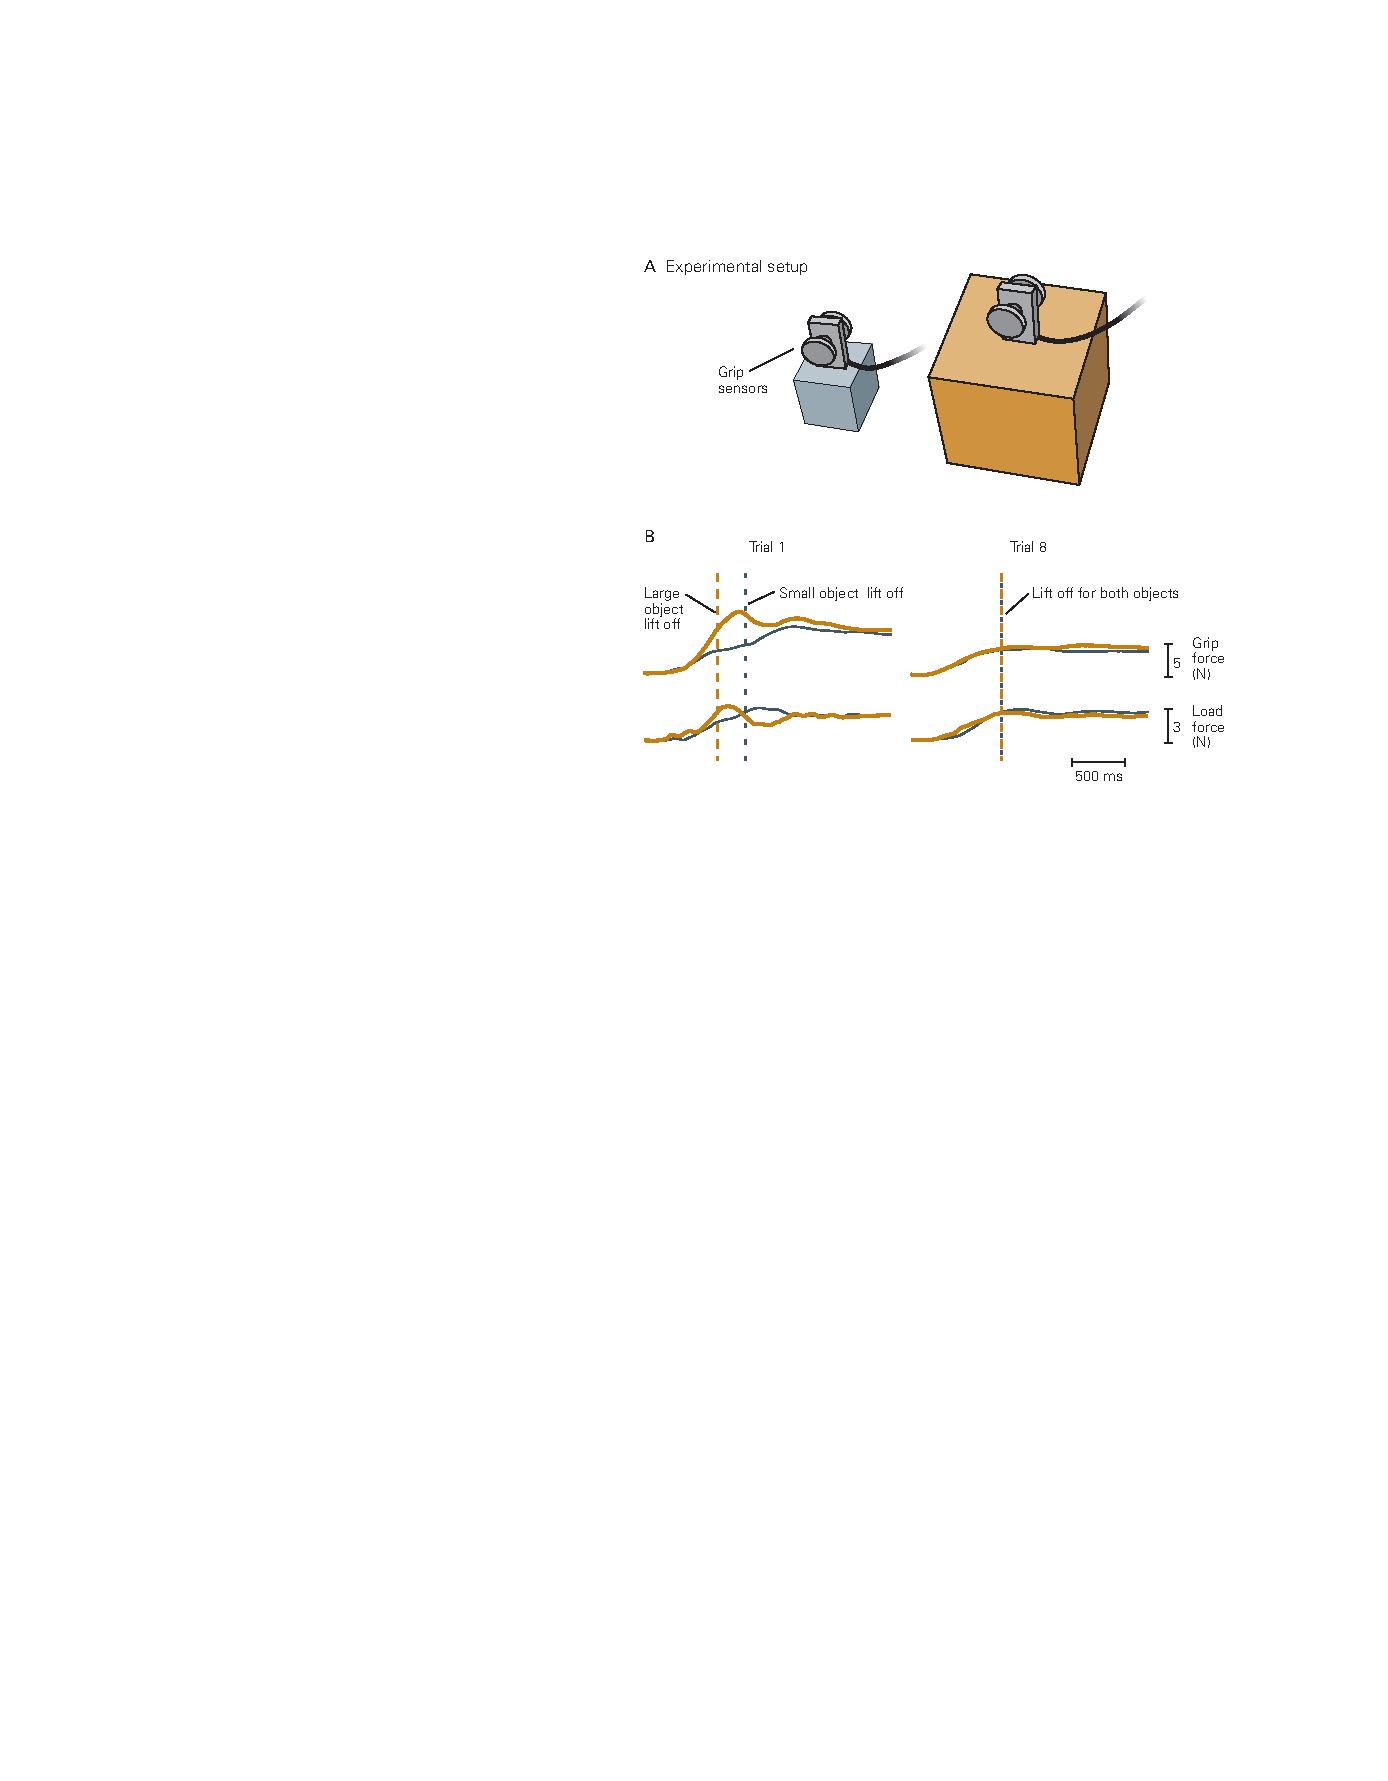
\includegraphics[width=1.0\linewidth]{chap30/fig_30_7}
	\caption{体积重量错觉。
		\textbf{A.} 在每次试验中,受试者交替举起一个大物体和一个重量相同的小物体。
		受试者认为较小的物体感觉比实际重。
		\textbf{B.} 在第一个试验中,受试者对较大的物体(橙色痕迹)产生更大的抓握力和负载力,因为预计它比小物体重。
		在第八次试验中,两个物体的抓地力和负载力相同,这表明尽管持续有意识地感知重量差异,但用于此动作的感觉运动系统会产生适合两个物体重量的抓地力和负载力\cite{flanagan2000independence}。}
	\label{fig:30_7}
\end{figure}



\section{运动计划将任务转化为有目的的运动}

现实世界的任务被表达为目标:我想拿起杯子、跳舞或吃午饭。
然而,动作需要详细说明由人体 600 多块肌肉驱动的运动的时间序列。
目标陈述与为实现该目标而招募特定肌肉的运动计划之间显然存在差距。



\subsection{许多动作都采用了刻板的模式}

运动系统以多种不同方式完成同一任务的能力称为冗余。 
如果完成任务的一种方法不切实际,通常会有替代方法。 
例如,伸手拿某个物体这一最简单的任务,可以用无数种方法来完成。


运动的持续时间可以从很宽的范围内自由选择,并且在给定持续时间的特定选择的情况下,手沿着路径的路径和速度曲线(即轨迹)可以呈现许多不同的模式。
即使选择一条轨迹仍然允许无限多的关节配置将手握在路径的任何给定点上。
最后,将手臂保持在固定姿势可以通过广泛的肌肉协同收缩水平来实现。
因此,对于任何机芯,都必须从众多备选方案中做出选择。


我们都选择以自己的方式前进吗?
答案显然是否定的。
个体重复相同的行为以及个体之间的比较表明,运动模式非常刻板。


刻板运动模式的不变性告诉我们一些关于大脑在计划和控制我们的行动时使用的原则。
例如,在伸手时,我们的手倾向于大致沿着一条直线路径移动,并且随着时间的推移,手速通常是平滑的、单峰的并且大致对称(钟形,图~\ref{fig:30_8})。
做直线运动的倾向是一大类运动的特征,考虑到肌肉会旋转关节,这令人惊讶。


\begin{figure}[htbp]
	\centering
	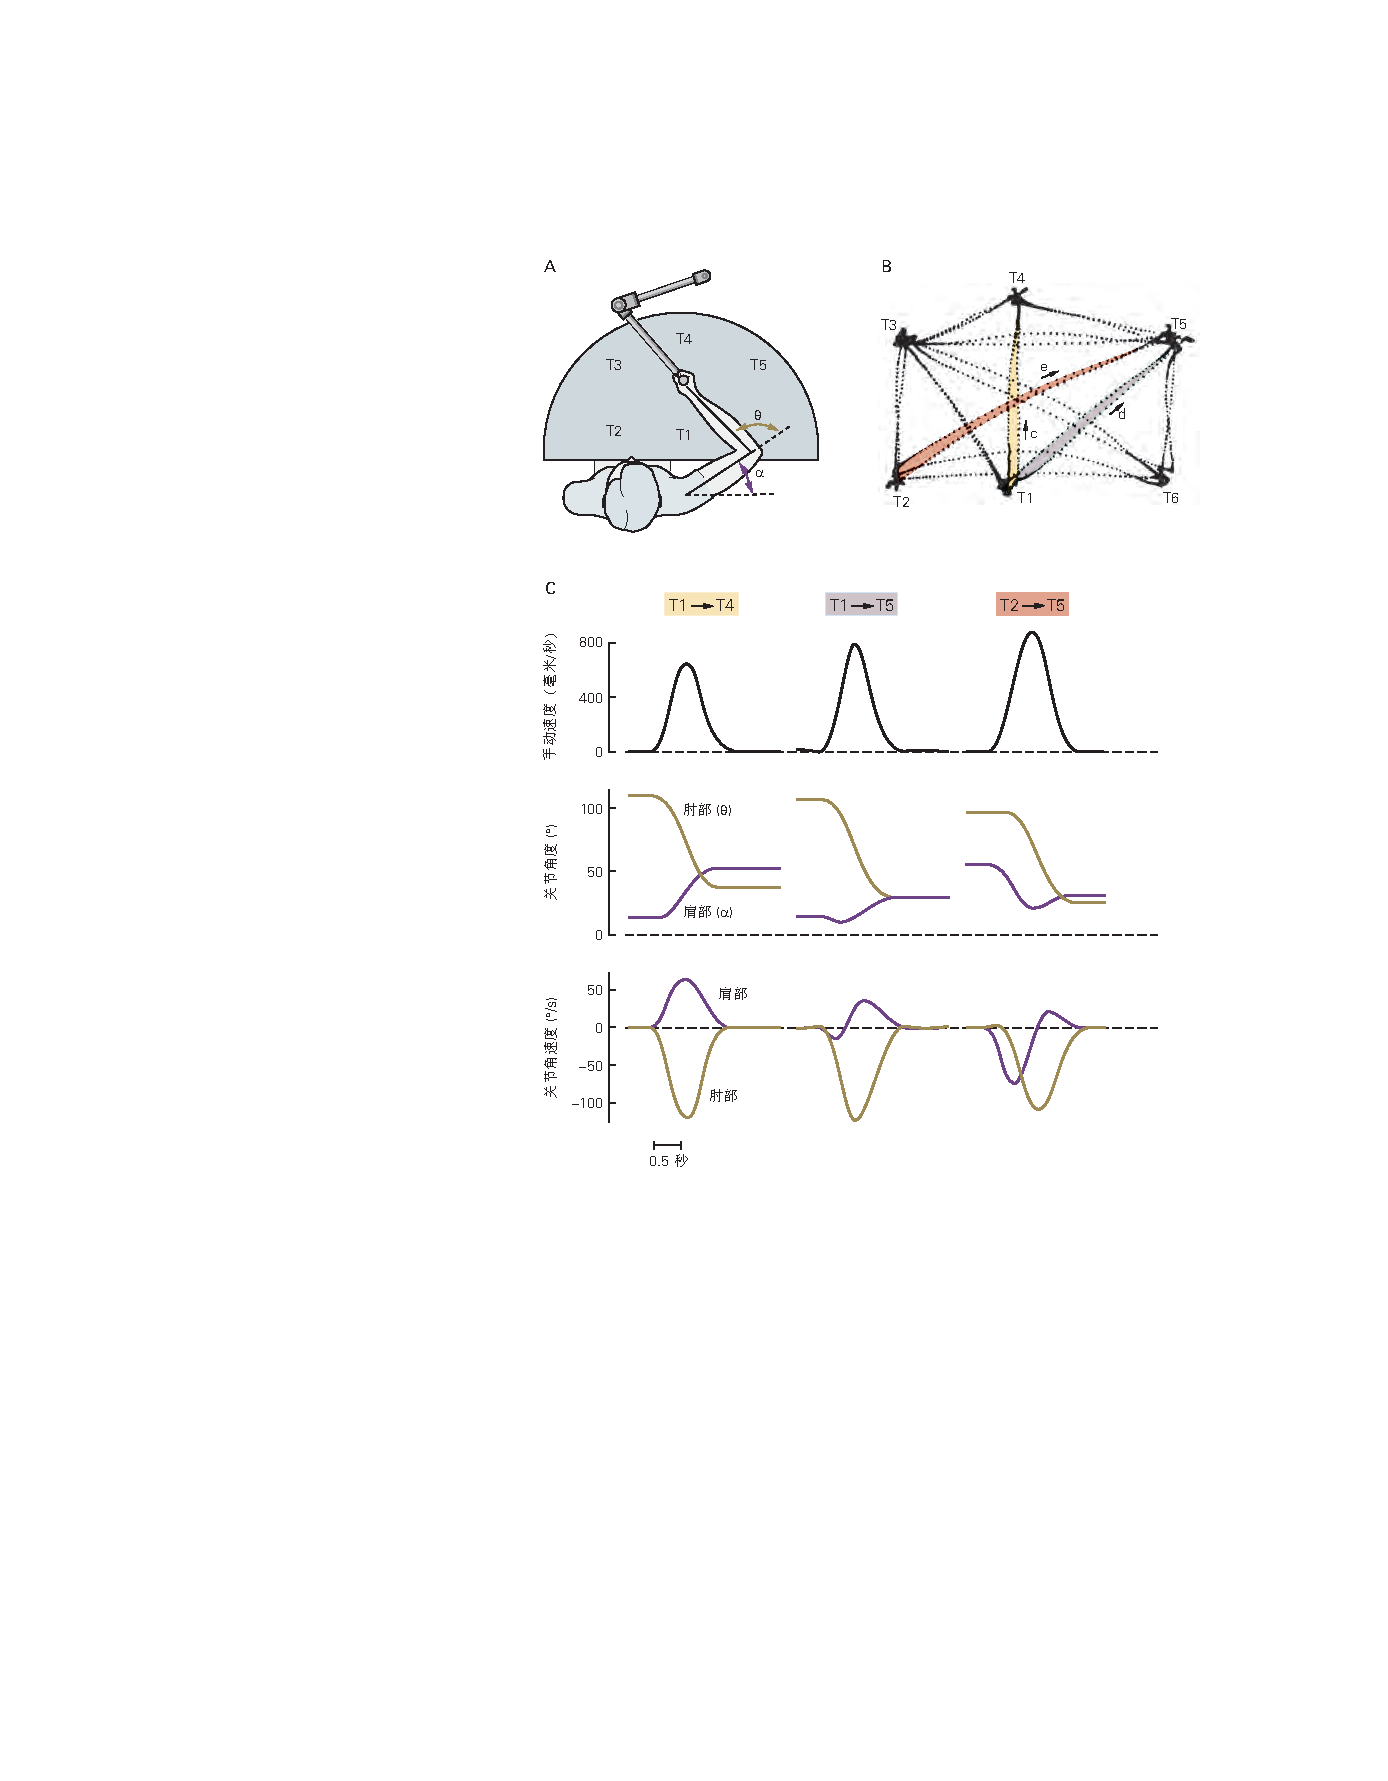
\includegraphics[width=0.88\linewidth]{chap30/fig_30_8}
	\caption{手的路径和速度具有定型特征\cite{morasso1981spatial}。
		\textbf{A.} 受试者坐在一个半圆形板前,抓住一个在水平面上移动并记录手部位置的双关节装置的手柄。
		指示受试者在各种目标(T1–T6)之间移动手。
		\textbf{B.} 一个对象在目标之间移动他的手时所追踪的路径。
		\textbf{C.} 面板 B 中显示的三个手部路径(c、d 和 e)的运动学数据。
		所有路径大致都是直的,并且所有手部速度曲线具有相同的形状和比例,与覆盖的距离成比例。
		相比之下,三个手部路径的肘部和肩部角速度分布不同。
		笔直的手部路径和速度的通用配置文件表明,规划是参考手部完成的,因为这些参数可以线性缩放。
		参考关节进行规划需要计算关节角度的非线性组合。}
	\label{fig:30_8}
\end{figure}


要实现手的这种直线运动需要复杂的关节旋转。
串联关节(肩、肘、腕)的运动非常复杂,并且随着初始位置和最终位置的不同变化很大。
由于单个关节的旋转会在手部产生弧形,因此肘关节和肩关节必须同时旋转才能产生直线路径。
在某些方向上,肘部比肩部移动得更多;
在其他情况下,情况恰恰相反。
当手从身体的一侧移动到另一侧时(图~\ref{fig:30_8},从 T2 移动到 T5),一个或两个关节可能必须在中途反转方向。
手轨迹比关节轨迹更不变的事实表明,运动系统更关心控制手,即使以产生复杂的关节旋转模式为代价。


这种以任务为中心的运动计划可以说明我们以不同方式执行特定动作(例如写作)的能力,但结果大致相同。
无论字母的大小或用于产生它的肢体或身体部分如何,手写体在结构上都是相似的(图~\ref{fig:30_9})。
这种称为运动等效性的现象表明,有目的的运动在大脑中是抽象表示的,而不是一组特定的关节运动或肌肉收缩。
这种能够驱动不同效应器的运动的抽象表示提供了一定程度的动作灵活性,这对于预设的运动程序来说是不切实际的。


\begin{figure}[htbp]
	\centering
	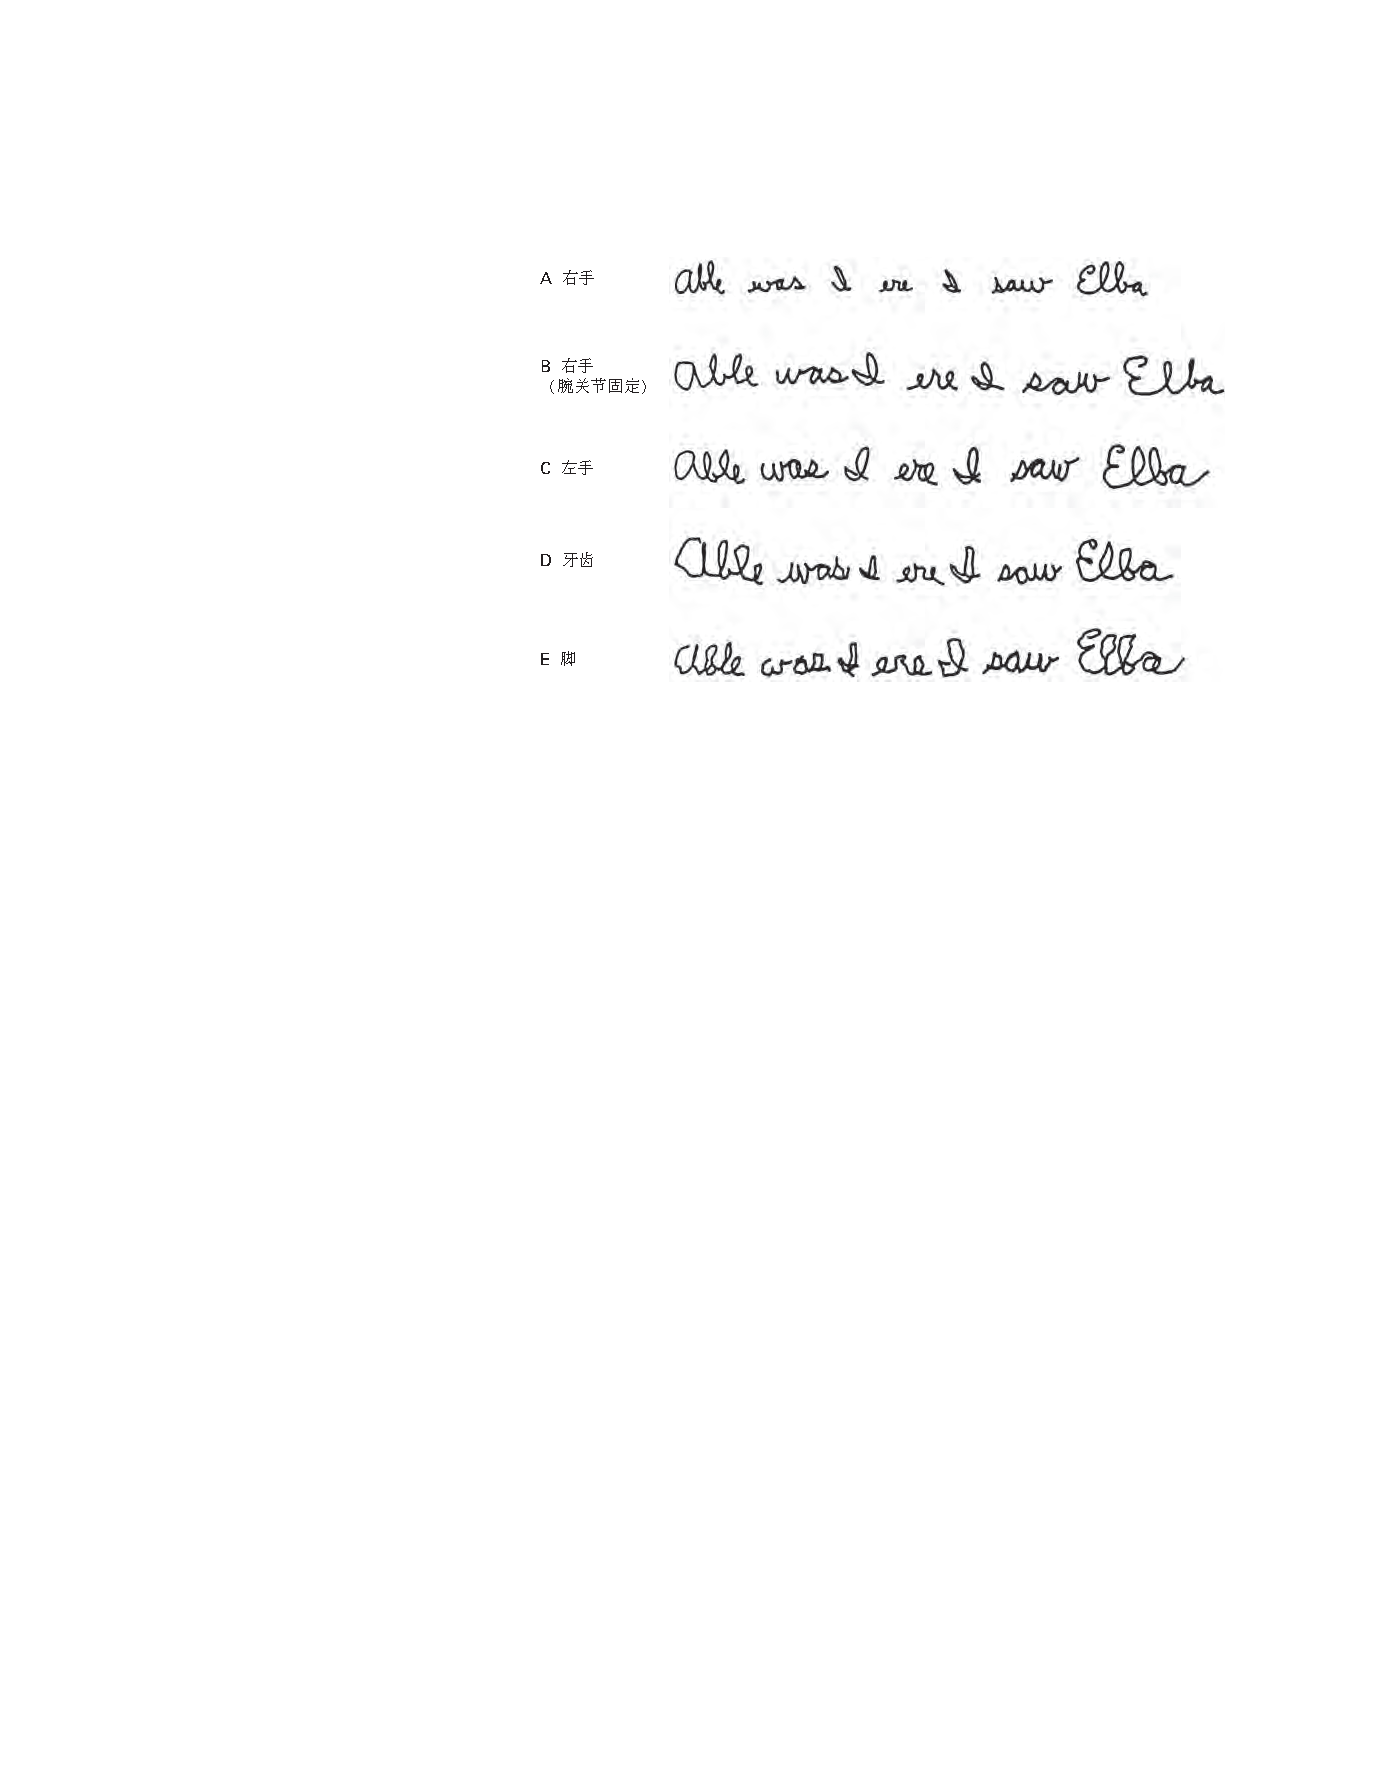
\includegraphics[width=0.73\linewidth]{chap30/fig_30_9}
	\caption{运动等效。
		不同运动系统实现相同行为的能力称为运动等效性。
		例如,可以使用身体的不同部位进行书写。
		此处的示例由同一个人使用右手(惯用手)(A)、手腕固定的右手(B)、左手(C)、咬在牙齿之间的笔(D)和附在脚上的笔(E)。}
	\label{fig:30_9}
\end{figure}



\subsection{运动规划可以是降低成本的最佳选择}

为什么人类会从无数种可能性中选择一种特定的方式来执行任务?
广泛的研究试图回答这个问题,已经出现的基本思想是,规划可以等同于选择完成任务的最佳方式。
在数学上,这等同于优化(即最小化)与运动相关的成本的过程。
成本是一种用单个数字量化机芯好坏的方法(例如,能量、准确性、稳定性)。


完成任务的不同方式会导致不同的成本。
这允许对所有可能的解决方案进行排序,从而确定成本最低的解决方案。
我们运动的不变性将反映我们关心的那种运动的特定成本。
已经提出了许多成本,但目前,大多数成功的理论认为运动成本有两个主要组成部分:任务成功和努力。
努力部分意味着我们希望以最少的精力成本取得成功。


要了解任务成功如何成为成本的组成部分,了解导致失败的原因是很有用的。
不准确的内部模型或处理显然限制了我们完成任务的能力,而运动学习旨在保持这些过程的准确性。
然而,运动系统中的低层组件(例如运动噪音)限制了成功。
运动往往是可变的,并且可变性往往随着运动的速度或力量而增加。
这种增加的部分原因是运动神经元的兴奋性和增加力量所需的额外运动单位的随机变化。
力的增量增加是由逐渐变小的运动神经元组产生的,每个运动神经元产生不成比例的更大的力增量(第~\ref{chap:chap31}~章)。
因此,随着力量的增加,运动神经元数量的波动会导致力量的更大波动。


通过要求受试者产生恒定的力,可以通过实验观察到这种情况的后果。
这种力量产生的可变性随着力量水平的增加而增加。
在大范围内,这种变异性的增加由恒定的变异系数(标准偏差除以平均力)捕获。
随着运动速度的增加(因为更快的速度需要更大的肌肉力量),这种对力的可变性的依赖性也增加了指向运动的可变性。
移动精度随着速度的增加而降低被称为速度-精度权衡(图~\ref{fig:30_10})。
这种关系不是固定的,部分技能学习,例如学习弹钢琴,涉及能够在不牺牲准确性的情况下提高速度。


\begin{figure}[htbp]
	\centering
	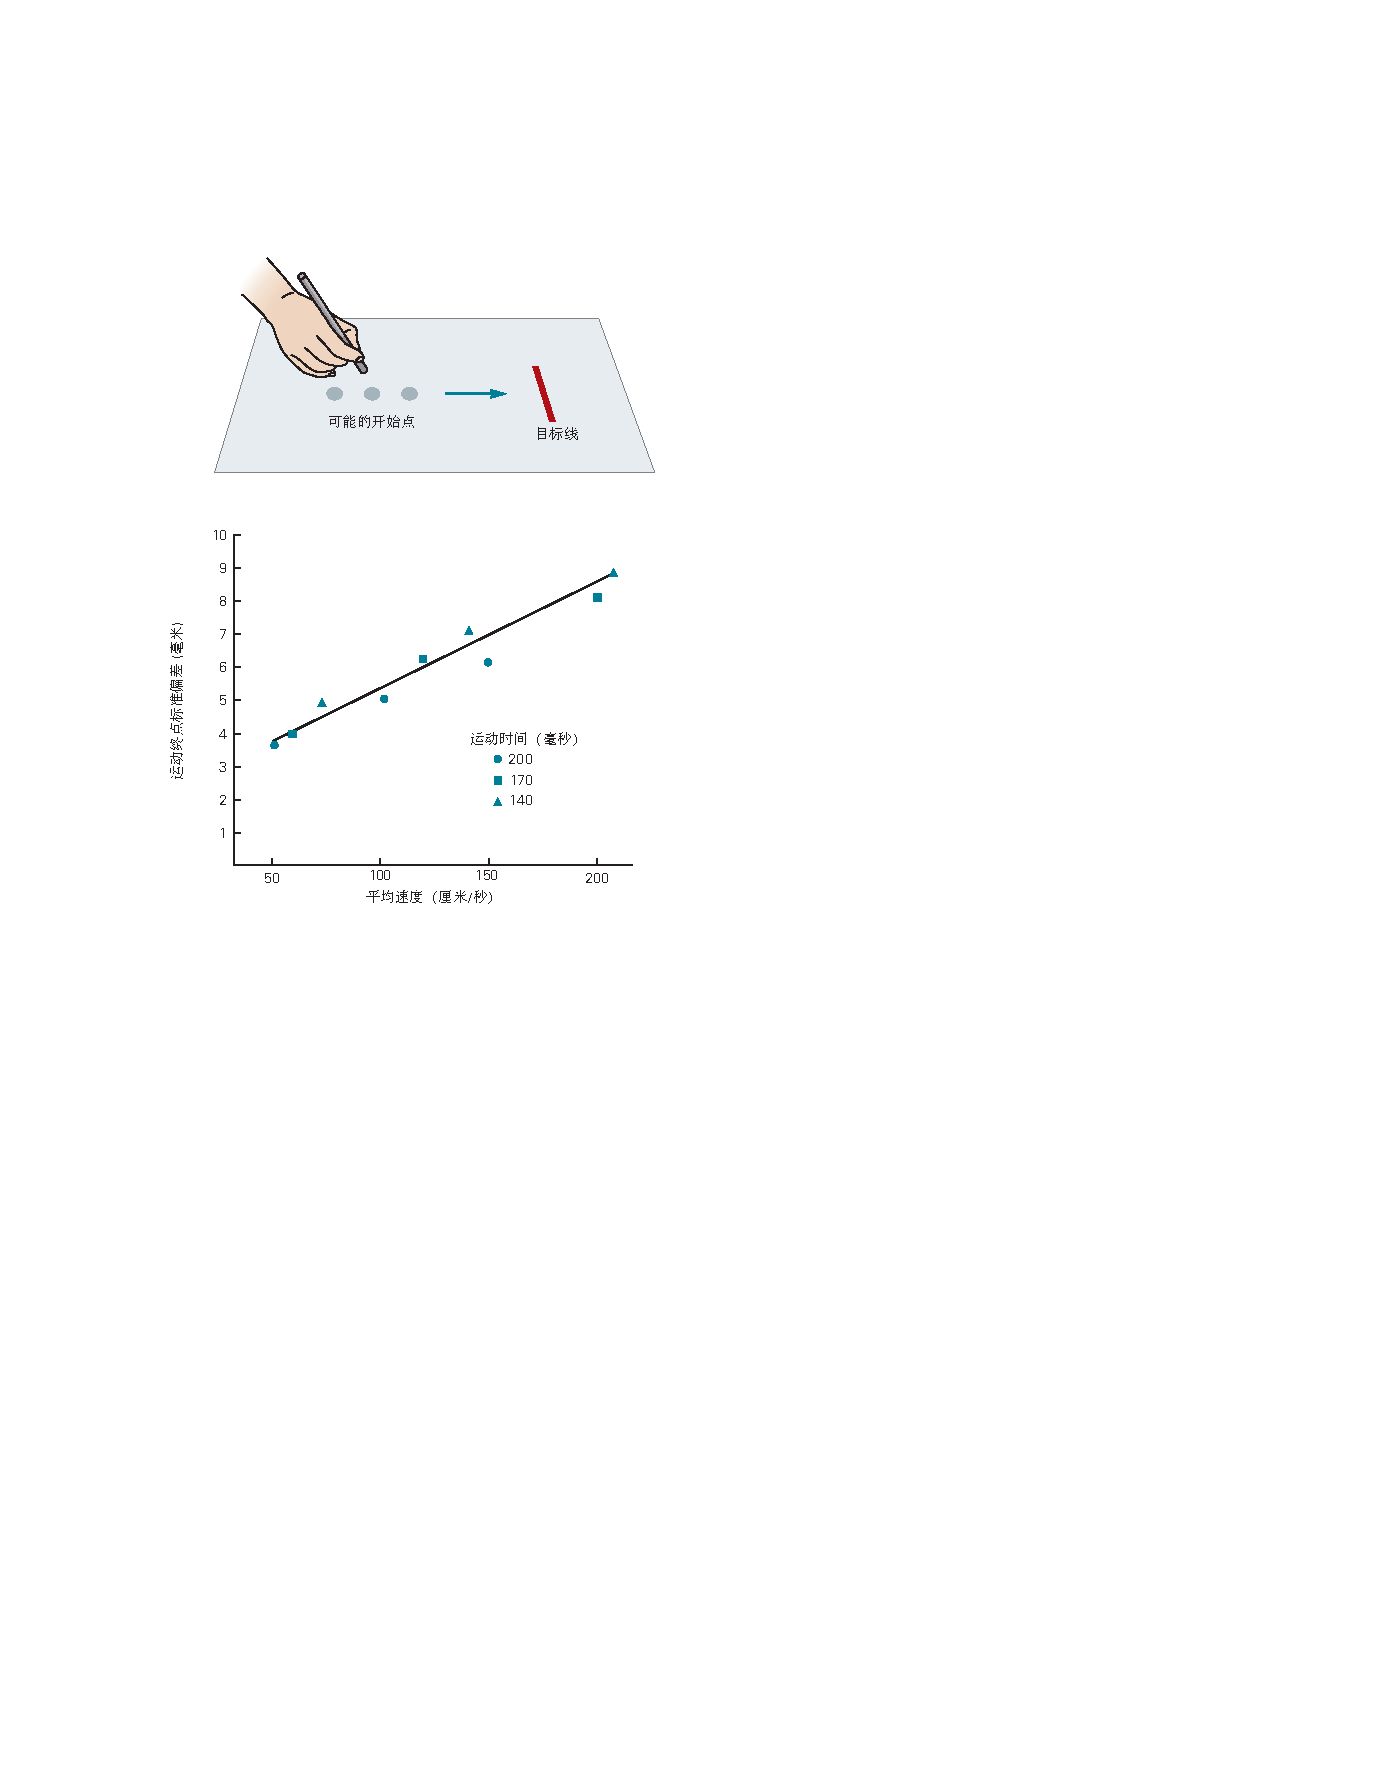
\includegraphics[width=0.6\linewidth]{chap30/fig_30_10}
	\caption{运动的准确性与其速度成正比。
		受试者拿着手写笔,必须击中一条垂直于他们移动手写笔方向的直线。
		受试者从三个不同的初始位置之一开始,并被要求在三个不同的时间(140、170 或 200 毫秒)内完成运动。
		如果受试者在要求时间的 10\% 内完成运动,则试验成功。
		只有成功的试验才用于分析。
		当试验不成功时,受试者会被告知。
		受试者手臂运动的变化在图中显示为运动终点的标准偏差与平均速度的对比(对于三个运动起点和三个运动时间中的每一个,给出九个数据点)。
		运动的可变性与速度成正比,因此与产生运动的力成正比\cite{schmidt1979motor}。}
	\label{fig:30_10}
\end{figure}


一般来说,努力和准确是矛盾的。
准确性需要能量,因为校正需要肌肉活动,因此需要付出一定的代价。
准确性和能量之间的权衡因不同的动作而异。
走路时,我们可以选择小心翼翼地迈步,以确保我们不会绊倒,但这需要消耗大量的能量。
因此,我们愿意让自己冒偶尔绊倒的风险来节省能源。
相比之下,在用刀叉进食时,我们会优先考虑准确性而不是精力,以确保叉子不会碰到我们的脸颊。


因此,最佳运动是在节能的同时最大限度地减少噪音的不良后果。
一种方法是指定一个理想的运动轨迹或可以被认为是最佳的状态序列。
虽然噪音和环境干扰会导致运动系统偏离预期的行为,但反馈的作用只是将运动恢复到预期的轨迹。
然而,这种方法在计算上不一定有效。
我们可以指定最佳反馈控制器来生成运动,而不是指定所需的身体状态。



\subsection{最佳反馈控制以任务相关的方式纠正错误}

最佳反馈控制旨在最小化成本,例如能量和任务不准确的组合(第~\ref{chap:chap34}~章)。
这种类型的反馈控制基于这样一种想法,即人们不会在给定特定成本的情况下计划轨迹。
相反,该成本用于创建一个反馈控制器,该控制器指定例如位置误差(以及速度和力等其他误差)的反馈增益如何随时间变化。
因此,给定任务目标,控制器指定适合身体不同可能状态的运动命令。
然后轨迹只是将反馈控制定律应用于身体状态的当前估计的结果(图~\ref{fig:30_11})。
反馈控制器是最优的,因为它即使在存在潜在干扰的情况下也可以最小化成本。


\begin{figure}[htbp]
	\centering
	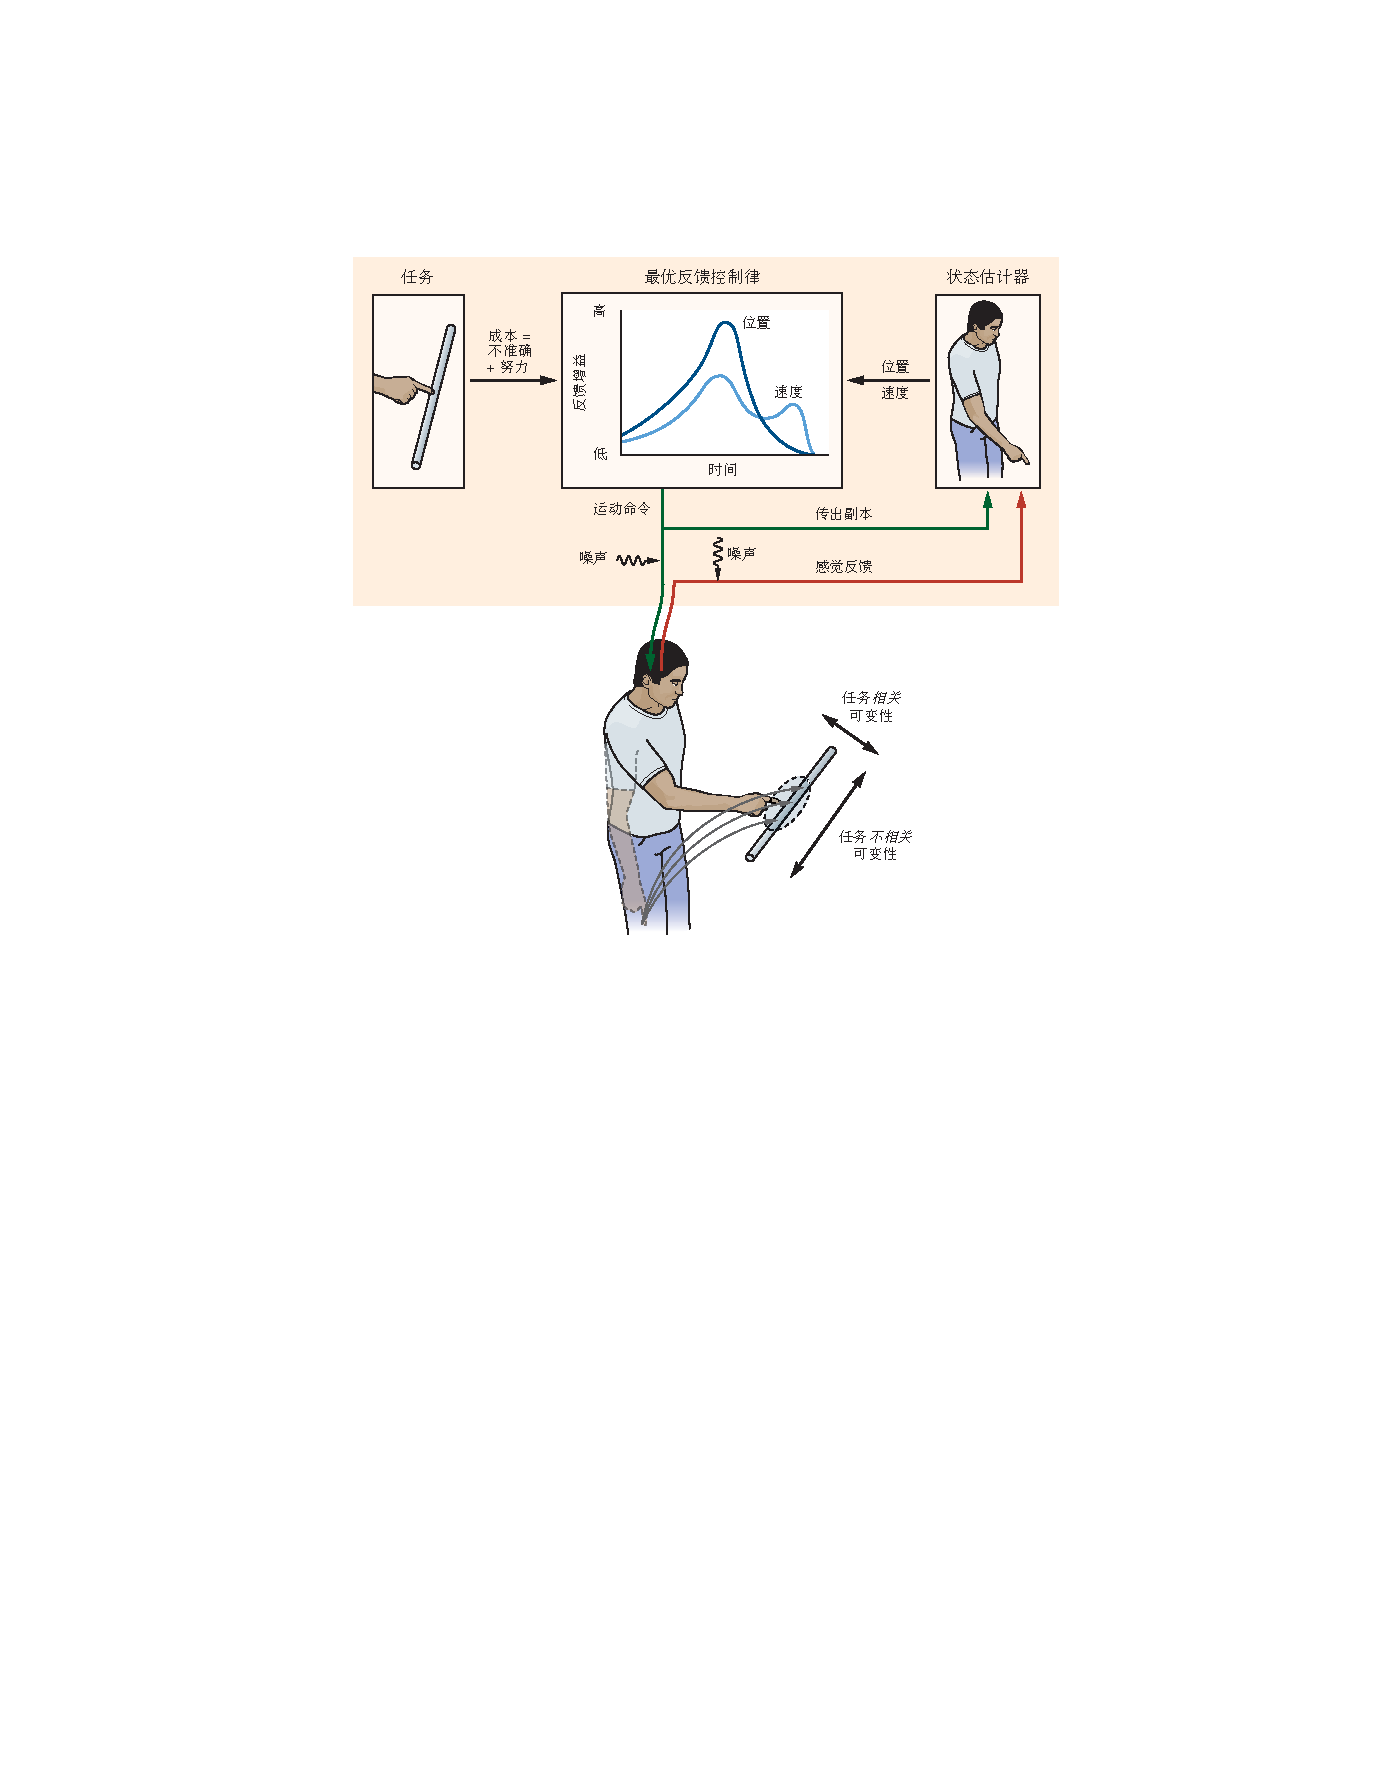
\includegraphics[width=0.82\linewidth]{chap30/fig_30_11}
	\caption{最佳反馈控制。
		为了针对给定的任务(例如触摸水平杆)生成运动,感觉运动系统指定了一个成本,该成本是准确性(例如,手指到杆的距离)和努力的组合。
		为生成使此成本最小化的运动,感觉运动系统设置了指定时变增益的最佳反馈控制规则。
		这些增益指定运动命令应如何取决于位置误差和手速度等状态。
		这种反馈控制法则的形式确保运动在存在内部噪声和外部扰动的情况下达到最佳状态。
		最佳行为倾向于让可变性(蓝色椭圆体,显示手可能的最终位置)在不影响任务成功的维度上累积(与任务无关的可变性),例如沿着条的轴,同时控制可能会发生的可变性 导致手错过了酒吧(任务相关的可变性)。
		显示了从同一起点到达的三个路径;仅在与任务相关的方面进行更正。}
	\label{fig:30_11}
\end{figure}


因此,最优反馈控制不会在前馈和反馈控制之间做出硬性区分。
相反,在一项任务期间,前馈和反馈控制之间的平衡沿着连续统一体变化,这取决于当前身体状态的估计受预测(前馈)或感官输入(反馈)影响的程度。


最佳反馈控制的一个重要特征是它只会纠正与任务相关的偏差,并允许与任务无关的偏差发生变化。
例如,当伸手去打开一个带有长水平手柄的出口门时,沿着手柄接触的位置并不重要,因此水平方向的偏差可以忽略不计。
这种考虑自然会导致最小干预原则,即只有在偏差会影响任务成功的情况下,才应该干预正在进行的任务。


干预通常会给系统增加噪音(并且需要付出更多的努力),因此不必要的干预会导致性能下降。
最佳反馈控制的目的不是消除所有可变性,而是允许它在不干扰任务的维度上累积,同时在与任务完成相关的维度上最小化它。
最小干预原则得到研究的支持,这些研究表明反馈并不总是使系统返回到未受干扰的轨迹,而是经常以一种方式起作用以减少干扰对实现任务目标的影响并确保纠正是任务-依赖。


最佳反馈控制强调反馈增益的设置,这可以通过产生快速运动响应的反射来部分实例化。
最佳反馈控制建议这些快速响应应该高度调整到手头的任务。
虽然短潜伏期(单突触)牵张反射仅对肌肉牵拉有反应,但人们早就知道长潜伏期反应对任务相关因素有反应(第~\ref{chap:chap32}~章)。
最佳反馈控制很重要,因为它结合了轨迹生成、噪声和运动成本,并为实验工作的结果提供了清晰的比较。



\section{多个过程有助于运动学习}

动物具有非凡的能力,可以通过与环境的日常互动来学习新的运动技能。
尽管进化可以硬连接一些先天行为,例如小马驹的站立能力或蜘蛛织网的能力,但需要运动学习来适应新的和变化的环境。


固定的神经系统无法获得新的运动技能。
随着身体尺寸和比例的变化,感觉运动系统必须在一生中不断适应,从而在运动命令和身体力学之间保持适当的关系。
此外,学习是获得社会习俗定义的运动技能的唯一途径,例如写作或跳舞。


大多数形式的运动学习都涉及程序性或内隐性学习,之所以这样称呼是因为受试者通常无法表达他们所学的内容。
内隐学习通常是在没有有意识地思考它的情况下发生的,并且可以在没有练习的情况下保留很长时间(第~\ref{chap:chap52}~章)。
程序学习的典型例子是学习骑自行车或弹钢琴。 相比之下,陈述性或显性学习指的是可以用关于世界的陈述来表达并且可用于内省的知识(第~\ref{chap:chap52}~章)。
记住脑神经的名称或去当地医院的方向是显性学习的例子。
陈述性记忆往往很容易被遗忘,尽管反复接触可以导致长期保留。
我们在最初学习一些运动任务时使用明确的学习策略,例如驾驶汽车,但随着时间的推移和练习,该技能会变得自动。


运动学习可以或多或少立即发生或随着时间的推移发生。
我们几乎是立刻就学会了拿起一个重量不明的物体,经过几周的练习我们学会了骑自行车,但掌握钢琴却需要数年时间。
这些不同的时间尺度可能反映了任务的内在难度以及执行任务必须忘记的进化限制。
例如,钢琴演奏需要学习对单个手指的精确控制,而在正常运动中,例如伸手和抓握,个性化的手指运动很少见。
感觉运动学习可分为两个广泛但重叠的类别:
适应感觉运动系统特性的改变和学习新技能。
我们依次关注每一个。



\subsection{基于错误的学习涉及适应内部感觉运动模型}

基于错误的学习是许多经过充分研究的感觉运动适应范式背后的驱动力。
例如,可以通过佩戴棱镜眼镜(甚至眼镜)来改变肢体的视觉位置和本体感受位置之间的关系。
这会改变视觉输入,从而使一个人伸手去拿某个物体的方向被误导。
通过反复尝试,调整到达轨迹以解决视觉和本体感觉之间的差异,这一过程称为视觉运动学习。
同样,要控制计算机鼠标,我们必须了解鼠标移动与屏幕上光标之间的运动学关系。
此外,肢体的特性会随着生长和工具的使用而变化。
大脑必须通过重组或调整运动命令来适应这些变化。


在基于错误的学习中,感觉运动系统感知每个动作的结果并将其与期望结果和预测结果进行比较。
例如,当投篮时,期望的结果是球穿过篮筐。
但是,一旦您放开球,您可能会预测球会偏向篮筐右侧。
预测和实际结果之间的差异,称为感官预测误差,可用于更新球如何响应您的动作的内部模型。
实际结果与期望结果之间的差异称为目标误差,可用于调整您的计划(即目标方向)以减少误差。
感官预测误差和目标误差对驾驶学习都很重要。


在将误差信号用于训练内部模型之前,可能必须对其应用额外的转换。
例如,当我们投掷飞镖时,视觉坐标会收到错误。
这种感觉误差必须转换为适合于更新控制过程(例如逆模型)的运动命令误差。
当运动系统学习新的感觉运动特性时,基于错误的学习往往会导致通过试验减少错误。


受试者可能会以两种方式中的任何一种来适应这种情况。
受试者可以共同收缩他们手臂的肌肉,从而使手臂变硬并减少扰动的影响,或者他们可以学习一个内部模型来补偿预期的力。
通过检查后遗症(机器人关闭后的动作),我们可以区分这两种学习形式。
如果手臂只是变硬,它应该继续沿直线移动。
如果学习了新的内部模型,新模型应该补偿不再存在的力,从而产生与早期扰动相反方向的路径。
在学习的早期,协同收缩用于在学习内部模型之前减少错误,但是随着内部模型能够补偿扰动,协同收缩随后会降低。
因此,当在学习后关闭力时,受试者通常会在相反方向显示出较大的后效应,表明他们已经补偿了扰动(图~\ref{fig:30_12}D)。


\begin{figure}[htbp]
	\centering
	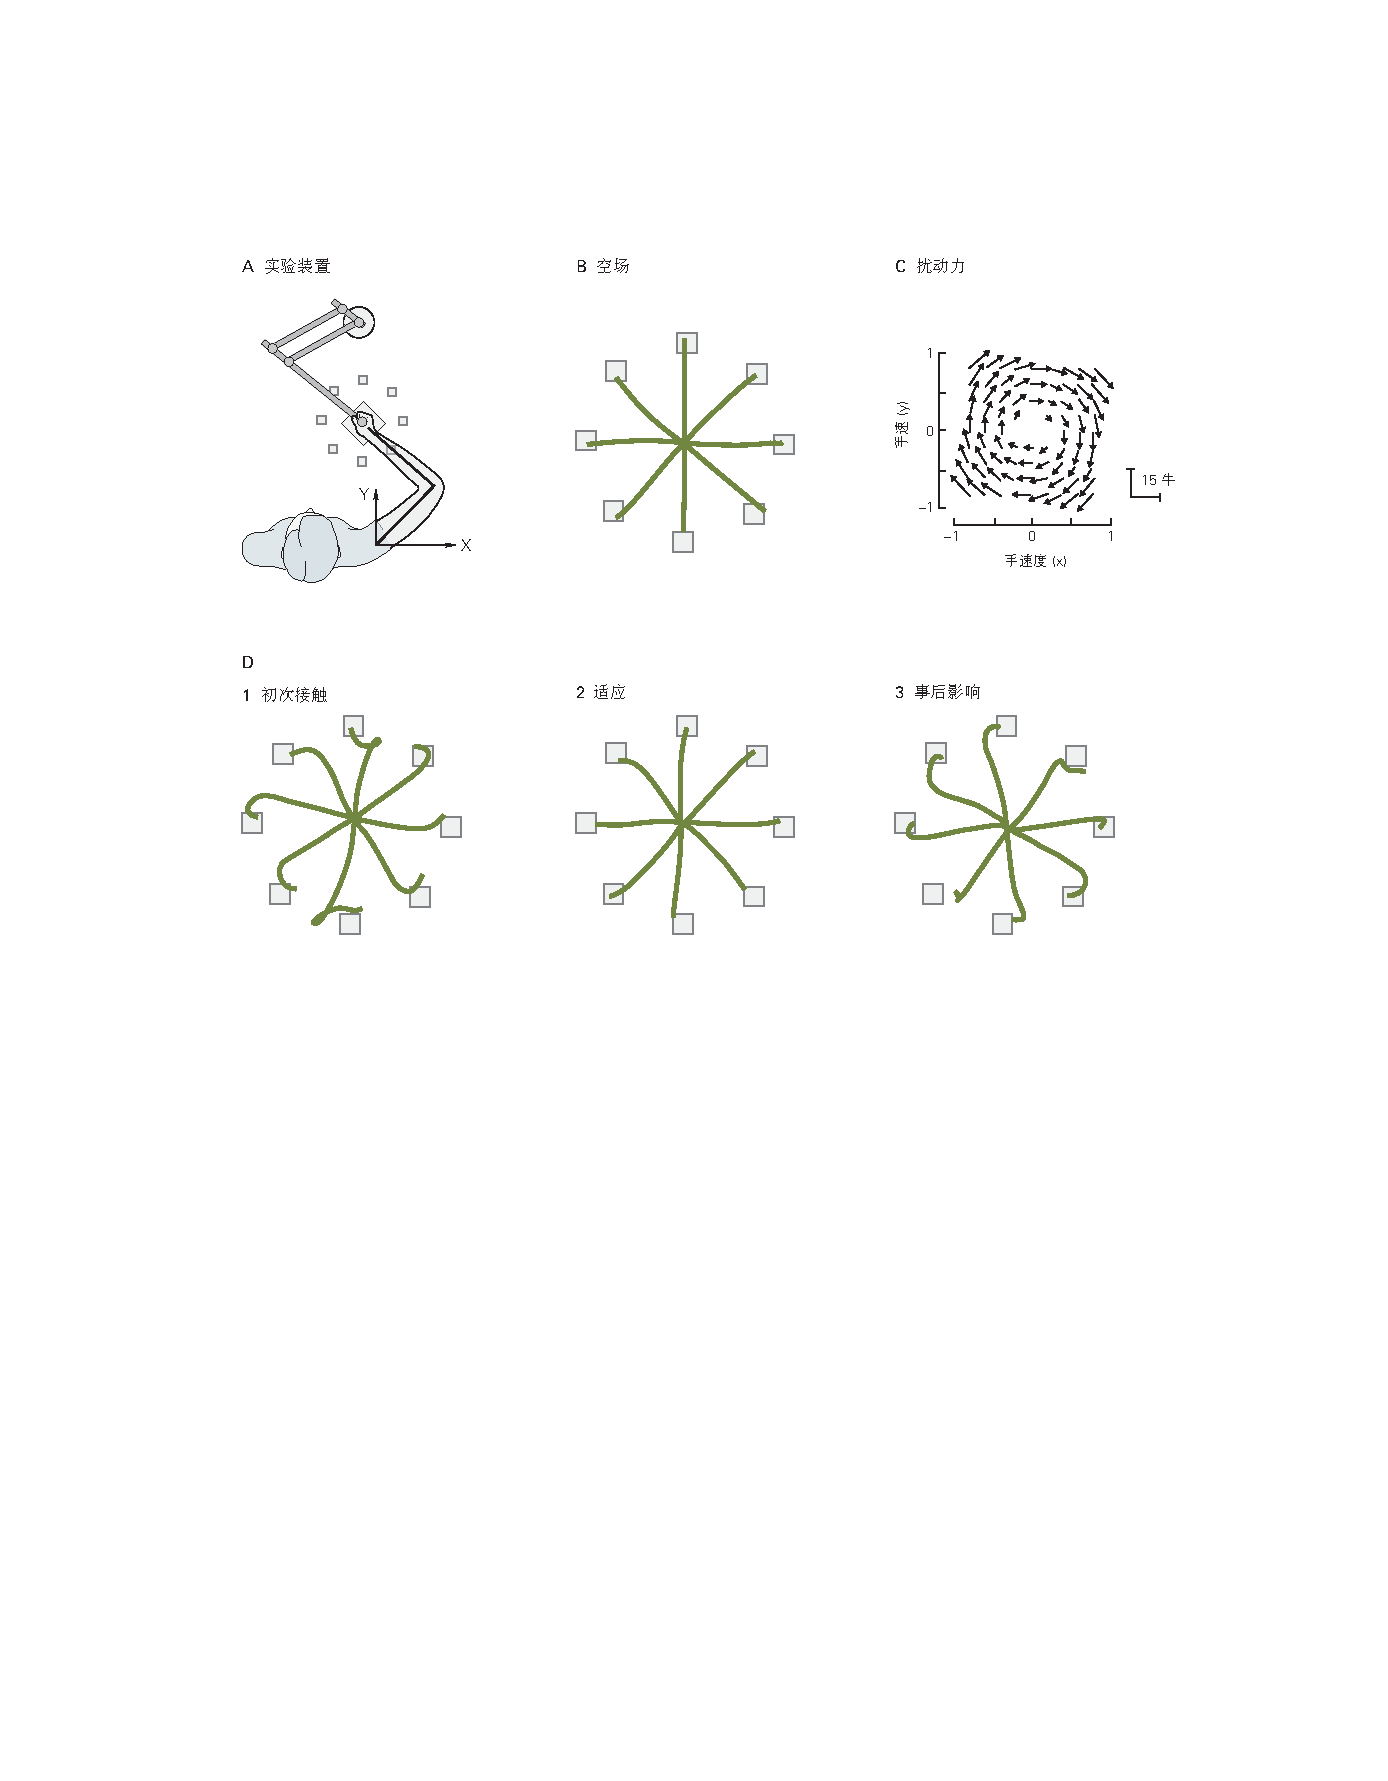
\includegraphics[width=0.98\linewidth]{chap30/fig_30_12}
	\caption{学习提高了在新的动态环境中到达的准确性\cite{brashers1996consolidation}。
		\textbf{A.} 受试者拿着一个机器人装置,该装置测量手的位置和速度并向手施加力。
		\textbf{B.} 当运动关闭时(空场),受试者从工作区中心大致直线移动到排列成圆圈的目标。
		\textbf{C.} 然后向手施加顺时针方向的力,显示为手速度的函数。
		该场产生与手的速度成正比的力,该力始终与当前运动方向成直角。
		\textbf{D.} 最初,手的路径受到扰动力(1)的响应而受到严重扰动。
		一段时间后,受试者适应并可以在整个运动过程中再次沿着直线路径移动(2)。
		当运动随后关闭时,运动再次受到扰动,但方向与先前的扰动相反(3)。}
	\label{fig:30_12}
\end{figure}


这种基于错误的过程似乎是许多不同运动类型和效应器(从眼睛到全身运动)适应的基础。
例如,我们正常的对称步态模式似乎依赖于基于错误的学习。
当受试者的步态模式因在一条皮带比另一条跑得更快的分体式跑步机上行走而受到干扰时,他们最初会跛行。
然而,逐步步态模式自然地恢复其对称性(图~\ref{fig:30_13}),从而表明基于错误的学习可以驱动复杂的全身协调运动。
有大量证据表明,基于试错的快速学习依赖于小脑(第~\ref{chap:chap37}~章)。


\begin{figure}[htbp]
	\centering
	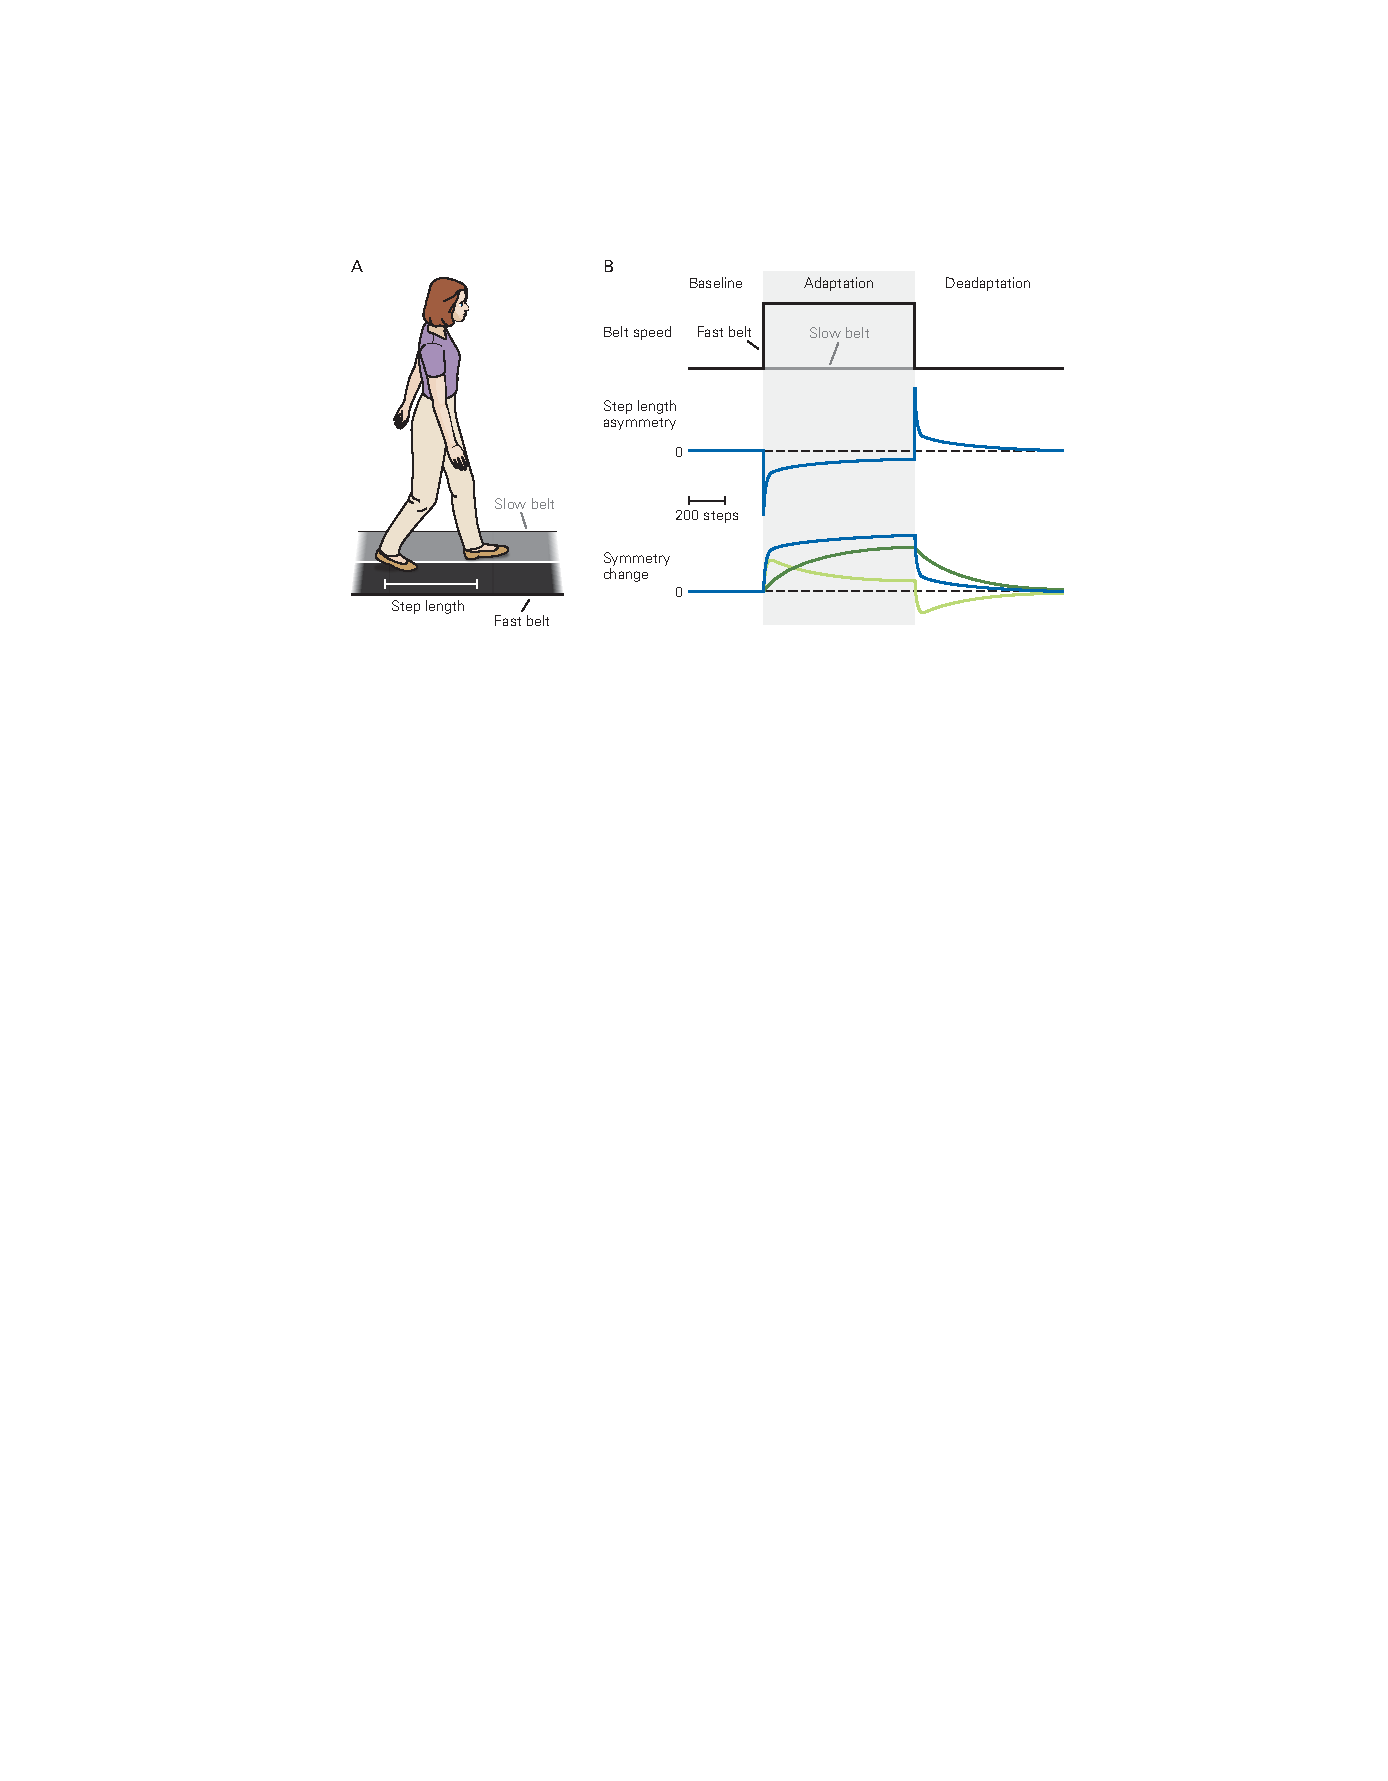
\includegraphics[width=0.88\linewidth]{chap30/fig_30_13}
	\caption{在行走中学习新的协调模式。
		\textbf{A.} 受试者在分体式跑步机上行走。
		当两条皮带以相同的速度移动时,受试者具有步长相等的对称步态模式。
		\textbf{B.} 在一项适应性研究中,皮带的速度最初是相同的,然后分开,使得右边的皮带移动得比左边的快,最后回到相同的速度(顶部)。
		当皮带以不同的速度移动时,步长对称性最初会丢失,导致受试者跛行。
		随着时间的推移,对称性恢复并且跛行被废除。
		当传送带再次以相同的速度移动时,可以看到后遗症(中)。
		\textit{莫里斯$\cdot$史密斯}及其同事表明,这种类型的适应由多个适应不同时间尺度的基础过程组成(底部)。
		步长对称性的变化由两个过程组成:一个快速过程(浅绿色线),适应速度快,但也很快忘记所学内容,一个缓慢过程(深绿色线),学习速度较慢但记忆力较好。
		这些过程都适应从错误中学习,这些过程的总和就是最终的适应(蓝线)。
		这种双速率学习系统产生了在许多适应形式中看到的典型双指数学习曲线,其中适应最初很快但随着学习的进行而趋于减慢\cite{roemmich2016seeing}。}
	\label{fig:30_13}
\end{figure}


运动适应可能不是一个单一的单一过程。
最近的证据表明,适应是由相互作用的过程驱动的,这些过程的输出是相结合的。
这些相互作用的过程可能具有不同的时间特性:
一个过程可以快速适应扰动,但也可以快速忘记所学内容,另一个过程学习速度较慢,但保留学习时间较长(图~\ref{fig:30_13}B)。
这种机制的优点是学习过程可以与扰动的时间特性相匹配,扰动的范围可以从短暂的(疲劳)到持久的(增长)。


尽管运动学习通常需要大量练习,但一旦不再执行某项任务,死适应通常会更快。
然而,与特定动作相关的感官输入足以改变行为。
例如,当受试者戴上可以改变视觉空间的棱镜眼镜时,他们最初在到达目标时会错过,但很快就会学会正确到达。
经过反复试验,在没有棱镜的情况下,仅凭眼镜的感觉就足以唤起适合棱镜的适应性行为。


一般来说,我们可以通过准确度和精确度这两个测量来量化性能。
准确性是衡量系统误差或偏差的指标,例如,一系列投掷的飞镖平均离目标有多远。
相比之下,精确度是衡量我们行为中的随机误差或统计变异性的指标。
准确度和精确度都有助于提高性能。
通常,可以通过调整或校准运动命令来提高精度,从而减少系统误差。
尽管不可减少的感觉和运动噪音总是会导致运动的一些可变性,但正如我们所见,可以通过计划减少可变性,从而将对任务成功的影响降到最低。
随着时间的推移,大多数运动学习趋向于自动(即隐性),但一些任务的早期学习可以通过显性学习(即策略)来辅助,例如关于如何最好地完成任务的口头指示。


并非所有感觉方式在学习所有运动任务时都同样重要。
在学习动态任务中,本体感觉和触觉输入比视觉更重要。 无论有无视觉,我们通常都能很好地学习动态任务。
然而,失去本体感觉和触觉输入的人特别难以控制四肢的动态特性或在没有视觉的情况下学习新的动态任务(方框~\ref{box:30_3})。


\begin{proposition}[本体感觉和触觉对感觉运动控制至关重要] \label{box:30_3}
	
	\quad \quad 虽然视觉障碍对感觉运动控制的影响肯定是有限的,但盲人能够正常行走,轻松地接触和抓住已知物体。
	这与本体感觉和触觉的罕见丧失形成了鲜明对比。
	
	\quad \quad 一些感觉神经病选择性地损伤外周神经和背根中携带大部分本体感觉信息的大直径感觉纤维。
	一个多世纪以来,本体感觉丧失导致的运动控制障碍一直困扰着神经学家和生理学家。
	对感觉神经病患者的研究为了解感觉和运动计划之间的相互作用提供了宝贵的见解。
	
	\quad \quad 正如预期的那样,这类患者失去了关节位置感、振动感和精细触觉辨别(以及肌腱反射),但疼痛感和温度感都得到了充分保留。
	患有周围神经病变的患者无法保持稳定的姿势,例如,拿着杯子或闭着眼睛站着。
	动作也变得笨拙、不协调和不准确。
	
	\quad \quad 随着患者学会用视觉代替本体感觉,功能可能会在几个月内恢复,但这种补偿仍然让患者在黑暗中完全丧失能力。
	其中一些困难反映了无法检测在看不见的运动中产生的错误,比如物体的重量与预期不同。
	
	\quad \quad 当患者试图做出快速方向反转的运动时,周围神经病变尤其会使人丧失能力。
	对这些运动过程中的关节力矩的分析表明,具有完整本体感觉的受试者预测节段间力矩,而没有本体感觉的人则没有这样做(图~\ref{fig:30_14})。
	
	\quad \quad 然而,同样的患者很容易适应剧烈的运动变化,比如在镜子里看手的时候画一幅画。
	事实上,他们的表现比正常受试者要好,也许是因为他们学会了用视觉引导自己的动作,而且因为他们缺乏本体感觉,所以在视觉和本体感觉之间没有任何冲突。
	
	\quad \quad 即使在正常受试者中,触觉输入在操作任务中的相对重要性也可以很容易地证明。
	闭着眼睛点火柴相对容易。
	然而,如果指尖被局部麻醉剂弄得麻木,那么即使在全视力下,这项任务也非常困难,因为火柴往往会从手指上滑落。
	
\end{proposition}


\begin{figure}[htbp]
	\centering
	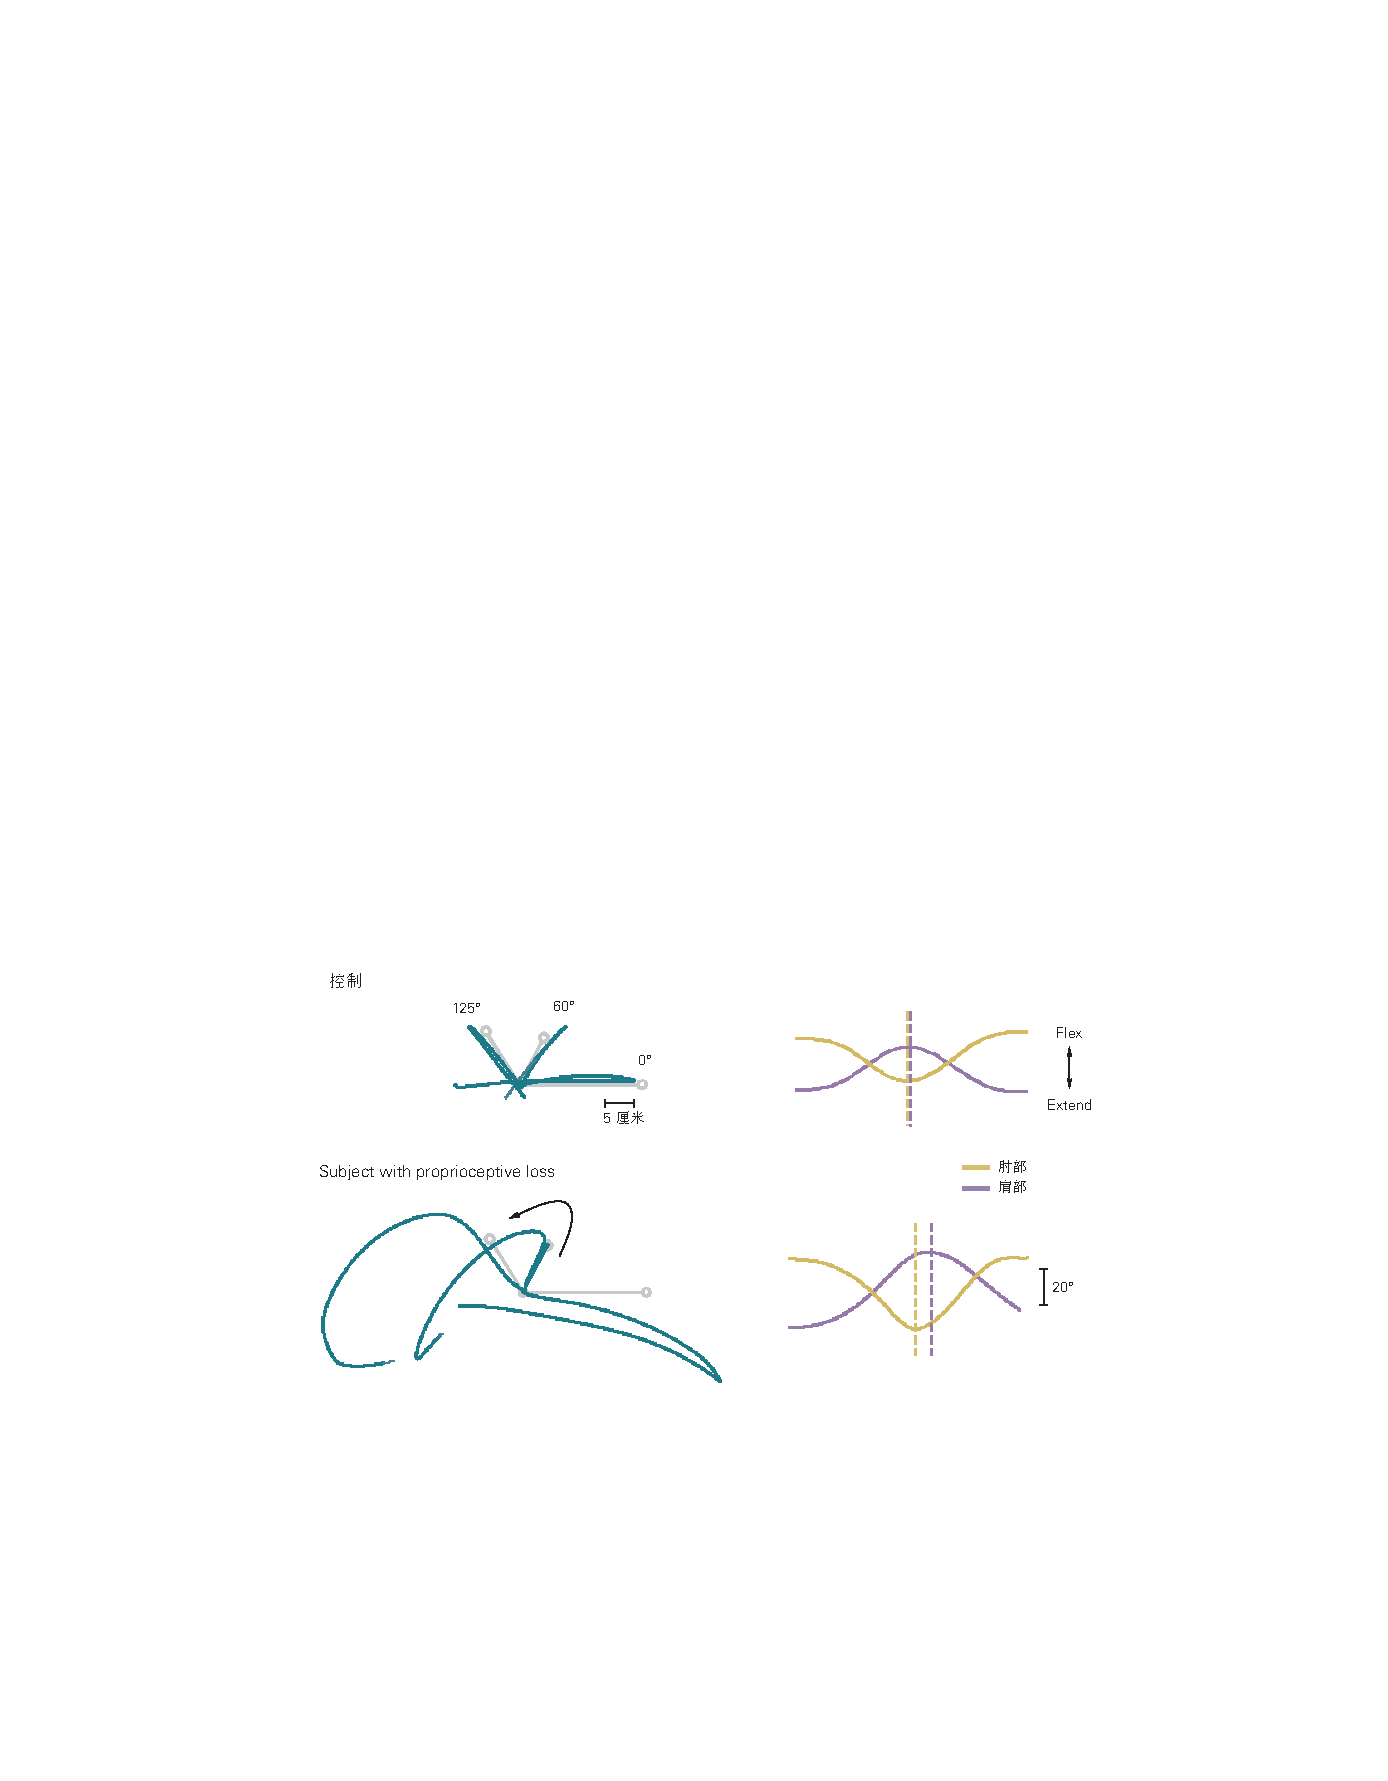
\includegraphics[width=0.85\linewidth]{chap30/fig_30_14}
	\caption{缺乏本体感觉的患者无法做出准确的运动,需要快速逆转路径。
		(左)受试者试图追踪一个模板(灰色线),而她的手被隐藏在视线之外。
		正常受试者的肘部和肩部的关节角度显示出良好的对齐(右上),从而导致准确的反转(左上)。
		相反,在缺乏本体感觉输入的受试者中,关节翻转的时机很差(右下),导致路径上的大误差(左下)。这些患者无法预测和纠正路径逆转周围发生的节段间动态。}
	\label{fig:30_14}
\end{figure}


\subsection{技能学习依赖于成功的多个过程}

与感觉运动系统适应扰动以恢复扰动前表现的基于错误的学习相反,系鞋带、杂耍、打字或弹钢琴等学习技能涉及在没有扰动的情况下提高表现。
这种学习往往会提高速度-准确性的权衡。
最初,我们可能能够以 1 秒的间隔敲击键盘上的正确键,但通过练习,可以以越来越快的速度达到相同的准确性。


对于某些技能,所执行的操作与任务的成功或失败之间可能存在复杂的关系。
例如,当孩子们第一次坐在秋千上时,他们必须学习使秋千变高所需的复杂的腿部和身体动作序列。
与基于错误的学习相比,没有现成的错误信号可用于调整当前动作,因为挥杆的高度不是由当前动作直接决定的,而是由身体和腿部运动的长期历史决定的。
在这种复杂场景中的学习可以使用强化学习来实现,在强化学习中,感觉运动系统调整其命令以努力最大化奖励,即任务成功。
在最一般的形式中,强化学习试图最大化的性能指标是所有未来奖励的总和。
然而,由于我们倾向于支持即时奖励而不是延时奖励,因此通常会对总和进行加权以通过逐步贴现未来奖励来反映这一点。


强化学习比基于错误的学习更普遍,因为训练信号是成功或失败,而不是每个时间点的错误。
强化学习的另一个显著特性是,学习系统的成功或失败可能以非平凡的方式取决于所采取行动的历史。
对于需要采取一系列复杂行动才能实现目标的任务,例如系鞋带,并且及时从行动中移除结果或奖励,不能轻易应用基于错误的学习。
强化解决的一个关键问题是信用分配问题:当我们最终成功或失败时,我们应该相信或指责序列中的哪个动作?
这正是强化学习算法擅长解决的问题。


强化学习主要分为两类,一类依赖于内部模型,另一类不依赖于内部模型。
基于模型的强化构建任务模型(例如,迷宫的结构)。
使用这样的模型,学习者可以以目标为导向的方式有效地进行计划。
相反,在无模型强化学习中,学习者只是将动作与成功或失败联系起来;
那些导致成功的人更有可能再次表演。
这种学习会导致运动习惯。
虽然无模型学习避免了构建模型的计算负担,但它也不太能够泛化到新情况。
这两种强化学习甚至可以一起作用,不同的任务可以不同程度地依赖它们。
基底神经节中的多巴胺能系统与人们在强化学习中预期的信号有关,例如预期奖励。
此外,这些系统的功能障碍与运动障碍、成瘾和其他可能与强化信号相关的问题有关(第~\ref{chap:chap38}~章)。


最后,有效策略的发展在运动技能习得中起着关键作用。
现实世界任务的技能学习通常涉及不同时空尺度的一系列决策过程。
例如,网球运动员的技术不仅取决于她击球的精确度,还取决于她能够正确决定将球瞄准何处的速度以及她运用感官的能力。
提取与任务相关的信息。



\subsection{感觉运动表征约束学习}

在一次运动中获得的信息通常太稀疏或太嘈杂,无法明确确定错误来源。
例如,如果网球运动员在发球时击球入网,问题可能是球抛得不够高、击球过早、球拍线松、有一阵风、 或者玩家疲劳了。
如果球拍的动态发生了变化,球员在下一次击球时会很好地适应这些变化。
如果问题是暂时的阵风,则无需调整。
为了解决这个问题,感觉运动学习系统限制了系统响应错误的更新方式。
这些约束反映了关于任务结构和错误来源的内部假设,并决定了系统如何表示任务。
事实上,在较慢的时间尺度上,学习本身可以改变表征。


虽然运动系统的最终输出是其 600 多块肌肉的收缩,但大脑并不是独立控制每块肌肉的。
在当前的感觉运动控制模型中,运动命令由多个模块生成,这些模块可以根据任务的要求有选择地参与。
模块化架构的示例包括多个内部模型、运动原语和运动协同作用(第~\ref{chap:chap36}~章)。


运动原语可以被认为是神经控制模块,可以灵活组合以生成大量行为。
基元可能表示特定肌肉活动或一组一起激活的肌肉的时间分布,称为协同作用。
整体运动输出将是所有原语的总和,由每个模块的激活级别加权。
然后,这些原语群体的构成决定了对学习施加哪些结构约束。
例如,运动系统具有许多原语的行为将很容易学习,而任何现有原语都无法近似的行为将无法学习。



\section{要点}

1. 大脑中发生的精细信息处理和存储的主要目的是使我们能够通过我们的运动系统与我们的环境互动。


2. 我们无限多样和有目的的运动行为受运动系统综合作用的支配,包括运动皮层、脊髓、小脑和基底神经节。


3. 为了控制动作,中枢神经系统使用了一系列感觉运动转换,将传入的感觉信息转换为运动输出。


4. 从快速反应到较慢的自主控制,不同级别的感觉运动反应的速度与复杂程度之间存在权衡。


5.运动系统使用前馈回路或纠错反馈回路产生指令;
大多数运动都涉及两种类型的控制。


6. 大脑使用感觉运动系统的内部模型来促进控制。


7. 使用感觉和运动信号以及前向预测模式来估计身体状态,以减少反馈延迟的不利影响。


8. 感觉输入和运动输出的可变性以及感觉运动转换的不准确性是运动误差和可变性的基础,导致速度和准确性之间的权衡。


9. 运动规划可以使用运动系统的冗余来移动,从而减少运动噪音的负面影响,同时减少工作量。


10. 运动控制回路不是静态的,而是在整个生命周期中不断修改和重新校准。


11. 运动学习改善新情况下的运动控制,不同形式的感官信息对学习至关重要。
基于错误的学习对于适应简单的感觉运动扰动尤为重要。
强化学习对于更复杂的技能学习尤为重要,它可以依赖模型(基于模型)或直接简单地强化运动动作(无模型)。


12. 大脑使用的运动表征限制了感觉运动系统在学习过程中更新的方式。


13. 感觉运动控制的研究侧重于深入了解相对简单的任务,例如伸手和走路。
尽管这些任务可以进行分析和建模,但它们并没有捕捉到真实世界运动控制的全部复杂性。
挑战在于确定这些原则是否可以推广到系鞋带和学习滑板等任务。


